\documentclass[a4paper,oneside,12pt]{book}
%----------------------------------------------------------------------------------------
%	WELCOME!
%----------------------------------------------------------------------------------------

%----------------------------------------------------------------------------------------
%----------------------------------------------------------------------------------------

\newcommand{\thesistitle}{Neural Network Optimization using Parallel Computing} 
\newcommand{\degree}{M.Sc. (High-Performance Computing)} 
\newcommand{\typeofthesis}{Master's Degree Project} 
\newcommand{\authorname}{Saumya Bhatnagar} 
\newcommand{\authorid}{16338296}
\newcommand{\keywords}{HPC, Neural Networks, Genetic Algorithm} % Keywords for your thesis
\newcommand{\school}{\href{https://www.maths.tcd.ie/}{School of Mathematics}} 


\AtBeginDocument{
\hypersetup{pdftitle=\thesistitle} % Set the PDF's title to your title
\hypersetup{pdfauthor=\authorname} % Set the PDF's author to your name
\hypersetup{pdfkeywords=\keywords} % Set the PDF's keywords to your keywords
\hypersetup{pdfsubject=\degree} % Set the PDF's keywords to your keywords
}

%% Language and font encodings
\usepackage[T1]{fontenc} 
\usepackage[utf8]{inputenc}
\usepackage[english]{babel}
\usepackage{longtable,lscape}
%% Bibliographical stuff
\usepackage[round,sort,comma,numbers]{natbib}

%% Document size
% include showframe as an option if you want to see the boxes
\usepackage[a4paper,top=2.54cm,bottom=2.54cm,left=2.54cm,right=2.54cm,headheight=16pt]{geometry}

%% Useful packages
\usepackage{amsmath}
\usepackage[autostyle=true]{csquotes} % Required to generate language-dependent quotes in the bibliography
\usepackage[pdftex]{graphicx}
\usepackage[colorinlistoftodos]{todonotes}
\usepackage[colorlinks=true, allcolors=black]{hyperref}
\usepackage{caption} % if no caption, no colon
\usepackage{sfmath} %use sans-serif in the maths sections too
\usepackage[parfill]{parskip}    % Begin paragraphs with an empty line rather than an indent
\usepackage{setspace} % to permit one-and-a-half or double spacing
\usepackage{enumerate} % fancy enumerations like (i) (ii) or (a) (b) and suchlike
\usepackage{booktabs} % To thicken table lines
\usepackage{fancyhdr}

\pagestyle{plain} % Embrace simplicity!


%\pagestyle{fancy}
%\fancyhf{} % sets both header and footer to nothing
%\renewcommand{\headrulewidth}{0pt}
%\cfoot{\thepage}
%\ifdefined\authorid
%\chead{\it \authorname\ (\authorid)}
%\else
%\chead{\it \authorname}
%\fi
%% End of block

\renewcommand{\familydefault}{\sfdefault} %use the sans-serif font as default


\renewcommand{\theequation}{\arabic{equation}} %% use continuous equation numbers

%% Format Chapter headings appropriately
\usepackage{titlesec}
\titleformat{\chapter}[hang] 
{\normalfont\huge\bfseries}{\thechapter}{1cm}{} 

\title{\thesistitle}
\author{\authorname}

\frontmatter
\begin{document}
\begin{titlepage}

\center % Center everything on the page

%% All the text parameters should be taken from the start of the main.tex file.
%% You should only alter stuff here if you want to change the layout

%----------------------------------------------------------------------------------------
%	LOGO SECTION
%----------------------------------------------------------------------------------------
%% Choose one of the following -- a colour or black-and-white logo


\includegraphics{title/Trinity_RGB_transparent_main.png}\\[1cm] 
%
\includegraphics[width=12cm]{title/black-stacked-trinity.jpg}\\[1cm] 

\Large \school\\[1.5cm] % Minor heading such as course title
\ifdefined\department
\large \department\\[1.5cm] % Minor heading such as course title
\fi

%----------------------------------------------------------------------------------------
%	TITLE SECTION
%----------------------------------------------------------------------------------------
\makeatletter
{ \huge \bfseries \thesistitle}\\[1.5cm] % Title of your document
 

%----------------------------------------------------------------------------------------
%	AUTHOR SECTION
%----------------------------------------------------------------------------------------

\ifdefined\authorid
\authorname\\ % Your name
\authorid\\[2cm] % Your Student ID
\else
\authorname\\[2cm] % Your name
\fi

%----------------------------------------------------------------------------------------
%	DATE SECTION
%----------------------------------------------------------------------------------------

{\large \today}\\[2cm] % Date, change the \today to a set date if you want to be precise

 
%----------------------------------------------------------------------------------------
%	TYPE OF THESIS SECTION
%----------------------------------------------------------------------------------------
 A \typeofthesis\ submitted in partial fulfilment\\of the requirements for the degree of\\
\degree

\vfill % Fill the rest of the page with whitespace

\end{titlepage}
\pagenumbering{roman}
\section*{\Huge{Declaration}}
\vspace{1cm}
I hereby declare that this project is entirely my own work and that it has not been submitted as an exercise for a degree at this or any other university.

\vspace{1cm}
I have read and I understand the plagiarism provisions in the General Regulations of the University Calendar for the current year, found at \url{http://www.tcd.ie/calendar}.
\vspace{1cm}

I have also completed the Online Tutorial on avoiding plagiarism `Ready Steady Write', located at
\url{http://tcd-ie.libguides.com/plagiarism/ready-steady-write}.
\vspace{3cm}

Signed:~\rule{5cm}{0.3pt}\hfill Date:~\rule{5cm}{0.3pt}

\chapter*{Abstract}
The rising importance of Artificial Intelligence and Machine Learning has demanded data scientists and researchers to discover new age computer systems that are capable of self-learning, reduce human effort and achieve high accuracy while performing tasks. The development of Artificial Neural Networks; a biologically inspired computing system, has emerged as one of the most effective solution to achieve this. The challenge, however, is optimizing Artificial Neural Networks to achieve high accuracy and speed. Given the vast selection of configuration variables (aka hyper-parameters), optimizing Neural Networks becomes a challenging and complex task. Various solutions to automate this task have since emerged. This thesis seeks to explore and compare the effectiveness of various methods that automate the Neural Networks optimizing process. An in-depth comparison between Genetic Algorithm, Parallel Genetic Algorithm and Quantum inspired Genetic Algorithm to optimize Neural Networks to achieve high accuracy and speed in processing Cifar-10 dataset has been presented in this thesis.


\newpage
\onehalfspacing\raggedright %\raggedright turns off justification and hypenation

\section*{\Huge{Acknowledgements}}

I would like to express my deepest appreciation to all those who provided me the possibility to complete this thesis. To begin, I would like to thank my dissertation supervisor, Dr. Darach Golden for his continual help, guidance and enthusiasm throughout the course of this research. It was through his supervision that I developed deep curiosity to dwell deeper into understanding Neural Networks and research effective new ways to optimize them. I would also like to thank my parents who taught me to strive for nothing short of ‘excellence’. This has been a period of intense learning, both academically and personally. Your contributions were invaluable. 


\tableofcontents
\listoffigures
%\listoftables
\newpage
%\section*{\Huge{Nomenclature}}
%\begin{tabular}{lp{9cm}l}
%A&Area of the wing&$m^{2}$\\
%B\\
%C& Roman letters first, with capitals\ldots\\
%a&then lower case.\\
%b\\
%c\\
%$\Gamma$&Followed by Greek capitals\ldots\\
%$\alpha$&then lower case greek symbols.\\
%$\beta$\\
%$\epsilon$\\
%TLA&Finally, three letter acronyms and other abbreviations arranged alphabetically\\
%\end{tabular}
%\vspace{2cm}


\mainmatter
\chapter{INTRODUCTION}

\section{Motivation}

The rise of the Fourth Industrial Revolution is characterized by the emergence of a fusion of technologies which are blurring the boundaries between the physical, digital, and biological realms \cite{schwab20164th}. Technologies such Artificial Intelligence, Machine Learning/Neural Networks and Quantum Computing have already begun to disrupt existing markets and value networks. The rising demand for these ‘new age’ technologies has enticed data scientists to focus efforts on developing more efficient accurate computing systems that have a wide application base. The advent of Neural Networks, a computing system that mimics the biological neural system of humans\cite{lippmann1987introduction}, has perhaps, been among the most important developments in the recent past.

The direct application of human nervous system into pattern recognition, aka "perception", has had a profound influence on the evolution of machine learning and artificial intelligence. Neural networks have been used to solve a wide spectrum of problems. Businesses and governmental organizations have used Neural Networks to facilitate sales forecasting, vehicular traffic identification, customer research, risk management and developing games for commercial use. Furthermore, this new age computing system has successfully applied to solve vehicular traffic identification, classifying images for human-computer interactions and for natural language processing, etc. 
The benefits of Neural Networks model are undeniable. However, a major factor limiting the use of Neural Networks in many cases, is the problem of achieving high accuracy and speed. The selection of configuration variables, a.k.a. “hyper-parameters”, helps optimize the accuracy and efficiency. A Neural Network continually attempts to readjust the hyper-parameters to fetch best results. Thus, hyper-parameter optimization is central to Neural Network modeling. Some business bet on hand tuning by experts. Researchers, however, have embarked on a journey to find method for automating the process.
A remarkable upgrade over the hand tuning method is the use of Genetic Algorithm (GA). Much similar to Neural Networks, the inspiration for GA finds its genesis in the biological sphere. GA uses a hybrid model of random search and generations. In this thesis, various concepts from GA such as exploitation of parents' features from previous generation to cross-breed, exploration in terms of randomly initializing population from the sample set based on the fitness of the population group \& mutation has been taken.

However, a major limitation of using GA is that the distant result of thousands of generations says very little about the effectiveness of the approach. To tackle the challenge of high computation cost of implementing evolutionary based optimization methods (e.g. in this thesis – genetic algorithm), parallel computing sweeps across the generations with minimal time, by creating parallel instances of the tasks. Depending on the job and resources, parallel instructions can be extended among nodes, cores or threads. Parallel computing has a strategic advantage of interdependence and/or independence of the parallel extension thus used. Parallel computing concepts can be borrowed by any programming language for staging concurrency. 

Irrespective of python’s versatile nature, with diverse libraries, innovative user interfaces, python has a reputation for being slow and unfit for High Performance Computing. Nonetheless, python being a competent language, has practical experience for scientific computing tasks. Fortunately, this research would comprehend the compatibility of python with HPC. Apart from multithreading and multiprocessing, python for parallel computing also characterizes MPI based parallel processing. Based on MPI-2 C++ bindings, module Mpi4py is python interface to MPI. \cite{dalcin2011parallel}. 
Expedition of deep learning contextually categorizing the hyper-parameters, adaptation of genetic algorithm for optimization, and erudition of Mpi4py, are therefore the key motivating factors behind this project.

\section{Research Question}
The rising importance of Neural Networks has undoubtedly caught the attention of an increasing number of data scientists and practitioners to find new application bases for the same. However, one of the major constraints during implementation is the tuning of hyper-parameters. Optimization is central to achieving high efficiency and accuracy of results.
Traditionally, hand/manual tuning of hyper-parameters had been the norm. However, in an attempt to find more effective methods for optimization, data scientists have zealously focused efforts on finding newer methods for achieving high accuracy and speed. This has given rise to several advancements in automated hyper-parameter tuning methods. While a host of optimization algorithms/methodologies exist, vast existing body of research shows GA\cite{stanley2002evolving} to be substantially more accurate and efficient in tuning Neural Networks. 

One major limitation, however, has been that Genetic Algorithms are slow. GA requires tens of thousands of generations to be run (which has proved to be a tenuous task). Implementation of Parallel computing could potentially be a solution to solve this problem. 

\textbf{The research question is:\\
How effective is Mpi4py\cite{dalcin2011parallel} based GA for optimizing Neural Networks to achieve both high accuracy and high efficiency on the Cifar-10 dataset? \\
}



While improvising Neural Network, exclusion of probable values for hyper-parameters may dominate poor performance. This thesis seeks to explore a methodology with all probable values in search space domain, hybridizing with concurrent scaling so as to avoid losing out on latency. 


\section{Research Objectives}
As highlighted in the previous sections, the overall purpose of this study is to present a comparison between the different ways of optimizing and parallelizing massive amounts of data using aggregated computing power. This facilitates in analyzing the performance of Mpi4py parallel programs and finally, determine what the best practices to be employed are. A overview of the goals and objectives of this research are presented below.

\begin{enumerate}
	\item To explore the impact of parallel computing
	\begin{enumerate}
		\item Present a comparison between Sequential and Parallel Computing.
		\item Compare Quantum inspired algorithm with Parallel Algorithm.
	\end{enumerate}
	\item To identify the best methods to parallelize computation process. Provide a comprehensive comparison between Mpi4py for 
	Single Population Fine Grained Algorithms and
	Multiple-population Coarse Grained Algorithms (Island Model)
	\begin{enumerate}
		\item Conduct performance analysis of the time taken to process the data
		\item Conduct performance analysis of accuracy achieved
	\end{enumerate}
	\item To highlight the impact of using different combinations of hyperparameters (using cifar-10 as input) on: 
	\begin{enumerate}
		\item accuracy
		\item time taken
	\end{enumerate}
	\textbf{The (a) Activation function (b) Optimizer (c) Number of Neurons (d) Number of layers and (e) Dropout have been taken as variables (hyperparameters).} 
	\item Overall, this thesis seeks to provide a recommendation for the best set of hyperparameters for initialization for cifer-10 dataset. 
\end{enumerate}


\section{Theory}

\subsection{Aspects of Neural Network}
With th advent of Neural Networks, there has been a resurgence in the field of High Performance Computing\cite{lippmann1987introduction}. Neural Networks have become of high importance to Machine Learning practitioners due to the wide spread computational application possibilities. Neural Networks can be used to rapidly provide a collectively-computed solution (a digital output) to a problem on the basis of analog input information \cite{hopfield1985neural}. Exploring the definition of Neural Networks provides a deeper insight onto how the computational system operates and provides promising results.

By definition, Neural Network computing architectures mimic the neuronal structure of the mammalian cerebral cortex. 

A Neural Network consists of a number of interconnected processing elements, commonly referred to as ‘neurons’ \cite{goh1995back}. The ‘neurons’ are arranged into multiple ‘layers’. Neurons within each layer are connected to and interact with neurons in the subsequent layers via ‘weighted connections’. The ‘weighted connections’ determine the level of influence between the interconnected neurons. A pictorial presentation of Neural Networks is presented in Figure 1.1. 

\begin{figure}
	\centering
	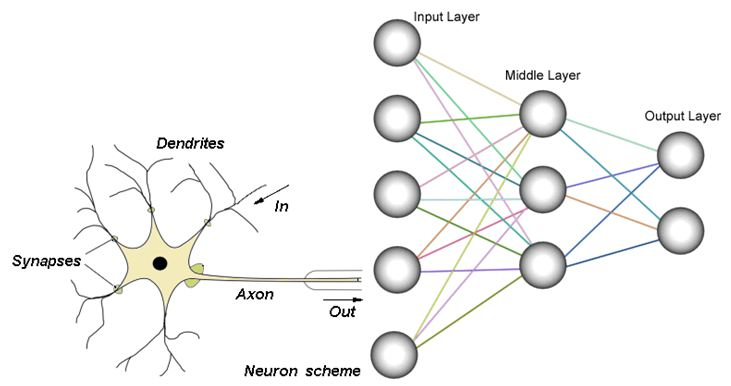
\includegraphics[width=1.0\columnwidth]{introduction/fig1a.jpeg}
	\caption{Biological vs Artificial Neuron, \href{https://54e779d2-a-62cb3a1a-s-sites.googlegroups.com/site/mrstevensonstechclassroom/hl-topics-only/4a-robotics-ai/neural-networks-computational-intelligence/Biological\%20vs\%20artificial\%20neuron.jpeg?attachauth=ANoY7cqMmj19FWvS5ZScxTm4AYPR7gp5OXR8mmegEe9VdE5N2pO_7KVYIA_oniPAsFBdG_Z2KIOIWWMZIhueb0m5EFIoE31mK9gl8UStTgYLeAyrMAYuqpNBTyGdRVSjx_5SgesKiyCP6wWhHptFr9_AhsTsXxuZbEjkCw45qyENjz2llQT8Fj-_vvPAnt8UyFXctSyLwadVcdv31CTNlLbjmLz6dekyA0aUR34gQMcoUMypraP9PlWZx988r4oOQzzQ2IbtD2JhHN5WZ42oww3UPK_Fk_otT5BmPieFdvAHXNuxX4MjEvV43HMsqAtfEJoLH1CC-mtDt94MsNARnSe_CJ7SrOSp9_EyuK_oSf_JLUQfRvBUwMM\%3D&attredirects=0}{source}}
\end{figure}


\begin{figure}
	% \centering
	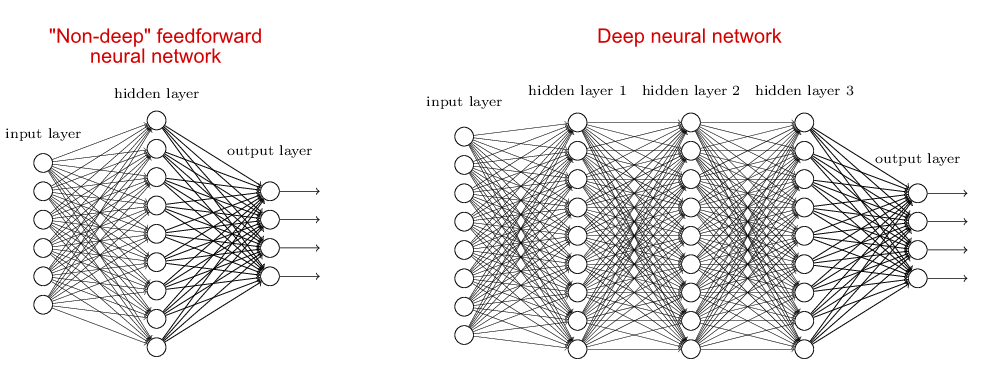
\includegraphics[width=1.0\columnwidth]{introduction/fig1b.png}
	\caption{Simple Neural Network vs Deep Learning Neural Network,
	\href{https://i.stack.imgur.com/OH3gI.png}{source}
	}
\end{figure}


As depicted in the Figure 1.2, Neural Networks consist of multiple layers. Signals pass from the input layer to the output layer. Data is presented to the input layer and the output layer holds the final responses. The “hidden layers” in between help represent and commute the association between the layers. 

One of the major benefits of Neural Networks is that they are capable of learning by adapting to the association of weights. Two strategies for training Neural Networks exist; \textbf{(i) Backward Propagation and (ii) Feedforward Neural Network training}. Webros’s\cite{werbos1974beyond} backward propagation algorithm significantly accelerated the training of Multilayer Networks by distributing the error term (or inaccuracy of fitting the Neural Network) back up through the layers. The error terms shrink exponentially as they propagate through layers. Deep Feedforward networks, also often called Neural Networks or Multi-layer perceptron (MLPs), are the quintessential deep-learning models. Feedforward Networks form the basis of many important commercial applications. For example, the Convolutional Neural Network (CNN) used for object recognition from photos are a specialized type of Feedforward network\cite{goodfellow2016deep}. Both MLPs and CNNs come within Deep Learning. Multilayer Perceptrons (MLPs) represent the most general Feedforward Neural Network model possible; they are organized in layers, such that every neuron within a layer receives its own copy of all the outputs of the previous layer as its input. The major difference between MLPs and CNNs is that CNN are less densely connected. This helps CNN scale down on the number of parameters through sharing of weights, conserving the information. Spatially close inputs are assumed to be correlated. For this reason, the accuracy gained through the use of CNN outweighs the accuracy derived through the use of MLP. The graphical representation of MLP and CNN is shown in Figure 1.3 and 1.4.

\begin{figure}
	\centering
	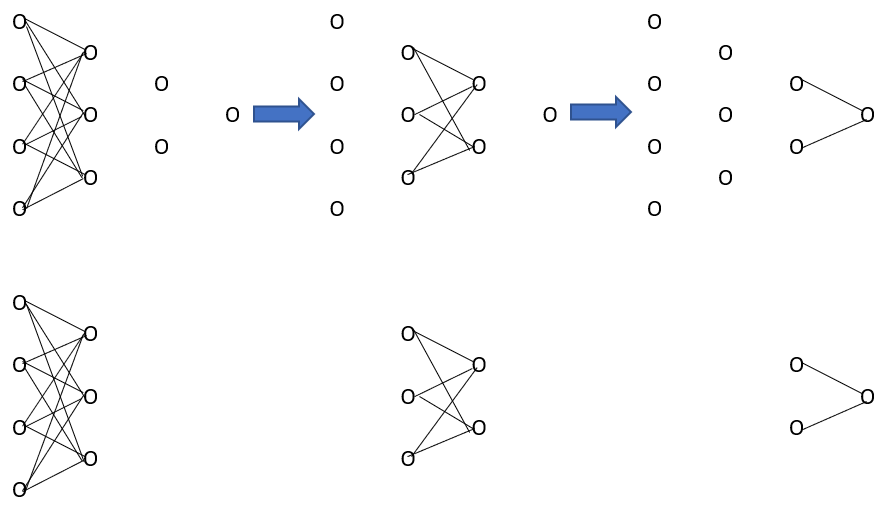
\includegraphics[width=0.8\columnwidth]{introduction/fig1c.png}
	\caption{Graphical Depiction of Multilayer Perceptrons}
\end{figure}


\begin{figure}
	\centering
	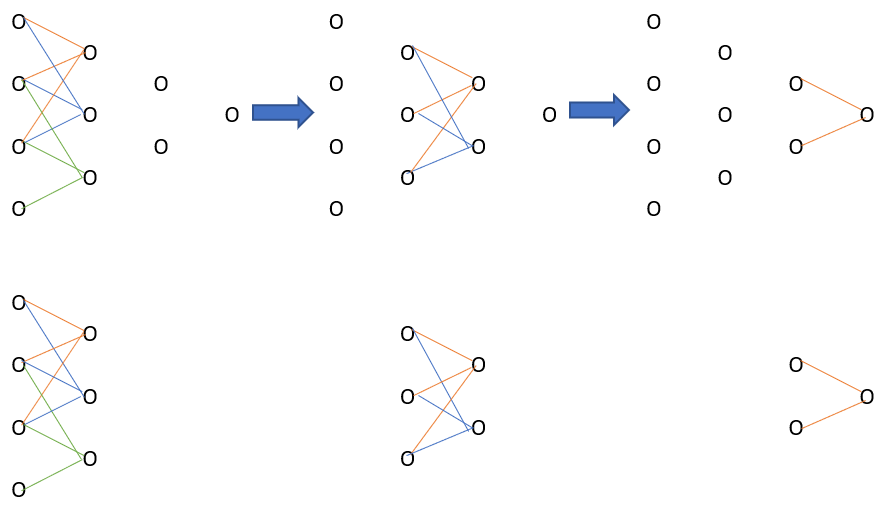
\includegraphics[width=0.8\columnwidth]{introduction/fig1d.png}
	\caption{Graphical Depiction of Convolutional Neural Networks}
\end{figure}

\textbf{Hyper-parameters }are variables which determine how the network is structured. In Machine Learning, Hyper-parameter Tuning or Hyper-parameter Optimization is the task of selecting a set of optimal parameters for solving an ML problem using a learning algorithm. Given the large number of ‘hyper-parameters’ which exist, choosing the appropriate architecture for achieving accurate results has remained as a subject of concern. Although many parameters exist, five parameters have been selected as configuration variables for the purpose of testing the results in this thesis. 
The structure of Artificial Neural Network is directly influenced by these parameters. Also, these parameters determine how the network is trained to achieve accurate results (thus, they are set before optimizing the weights and bias). A few other examples of parameters include learning rate and loss function.


\subsection{Survival of the fittest}

The previous section had introduced Convolutional Neural Network Model. This section seeks to provide an overview of the optimization technique used with brief detailing on the concepts of Genetic Algorithm (GA) that are used. 


Genetic Algorithms (GA) is an evolutionary algorithm inspired by Charles Darwin’s (1859)\cite{darwin2004origin} Theory on Natural Selection and Genetic Mutation. Darwin’s Theory of Natural Evolution points to premise that all species of organisms arise and develop through the mechanism of natural selection and genetic mutation. Organisms develop through a series of small, inherited variations that eventually improve the organism's ability to compete, survive, and reproduce. This is the basis of GA - a population-based metaheuristic optimization algorithm. Thus, Genetic algorithms can be applied to generate high quality solutions to optimization and search problems by relying on bio-inspired operators such as mutation, crossover and selection\cite{mitchell1998introduction}. 

In this thesis, the optimization technique is based on Natural Selection, Cross-Breeding over generations. The optimization technique - \textbf{EETO (Exploration \& Exploitation Trade-off based Optimization) method} makes use of the concepts inspired by GA to optimize the Neural Net as detailed below:

\begin{enumerate}
	\item Initialization of Parents' Genes: In the first step, random candidate solutions (parents' features/ chromosomes) are generated. These chromosomes are further used to breed/produce new populations.
	\item Iterative Generations: GA takes an iterative process where a sequence of outcomes is continuously developed until an optimal solution is provided. A population within each iteration is referred to as a ‘generation’.
	\item Fitness Evaluation: The ‘quality of the solutions’ is represented as ‘fitness’. Candidates of solutions are developed through evolution at each generation. The relative ‘fitness’ of the candidate solutions is expected to be higher through passing generations.
	\item Breeding: Breeding takes place after ‘Fitness Evaluation' and involves two concepts:
	\begin{enumerate}
		\item \textbf{Exploitation}: This step is based on 'Natural Selection'. Set of candidates are selected within each ‘generation’ based on ‘fitness’. Relatively ‘fitter’ solutions are selected from previous generations. During 'Crossover', the algorithm exploits the features of the selected parents to generate a new offspring. There are multiple methods of crossovers. In a single point crossover, only one crossover point is selected in contrast with multi-crossover point. This thesis uses Uniform Crossover. A Uniform Crossover point randomly selects from the parents. In contrast, under Arithmetic Algorithm, arithmetic operations are performed to produce off-springs. A graphical representation of these algorithms is presented in Figure 1.5.
		\item  \textbf{Exploration}: This step involves killing/deleting the least fitting individual and re-initializing the individual randomly ensuring exploration to get out of local maxima and produce optimal solutions by reaching global maxima. 
	\end{enumerate} 

	\begin{figure}
		% \centering
		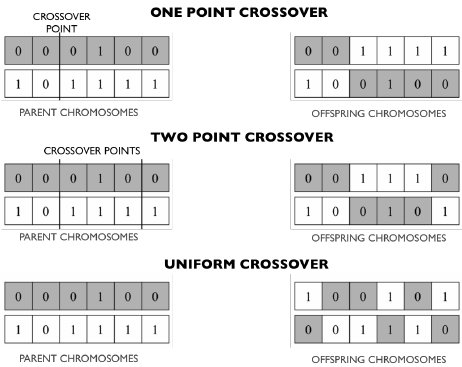
\includegraphics[width=1.0\columnwidth]{introduction/fig1e.jpg}
		\caption{Types of crossover,
		\href{https://www.researchgate.net/publication/268525551_Genetic_Algorithms_in_Wireless_Networking_Techniques_Applications_and_Issues/figures?lo=1}{source}
		}
	\end{figure}
	\item Mutation: Each candidate solution has a set of properties (its chromosomes or genotype) which can be mutated and altered; traditionally, solutions are represented in binary as strings of 0s and 1s, but other encodings are also possible\cite{whitley1994genetic}. It is important noting that the mutation rate can influence the convergence. A sub-optimal mutation rate could lead to a ‘Genetic Drift’. A Genetic drift is the change in the frequency of an existing gene variant (allele) in a population due to random sampling\cite{masel2011genetic} of the off-springs (candidate solutions). Genetic Drift plays a mirror role in the evolution process. In case of slow mutation rate, Genetic Variation is likely to be reduced, causing reduced incremental rate of ‘average fitness’ through passing generations. On the contrary, a suboptimal ‘high mutation rate’ increases the risk of good solutions being lost. 
	\item Termination: The final step is termination. Termination is normally achieved when the iterative process can no longer continue. In this thesis, the termination circumstances that are considered are listed below:
	\begin{enumerate}
		\item Number of generation constraints
		\item In case if outcome satisfactory meets the minimum criteria.
	\end{enumerate}
\end{enumerate}




\subsection{Quantum Computation}
In classical computers information is stored in bits(0 or 1). However, in a quantum computer, the information is stored in qubit, building block of a quantum computer, which is a spin-1/2 of particle such as a proton, neutron, or electron. So, a quantum memory register is composed of several spin-1/2 particles, or qubits. A qubit stores a superposition of 0 and 1, after measurement the state collapses from it's superposition state to one of these two states. 

While in a superposition state, a qubit can take any value between 0 and 1. This increased sample space is the key to evaluate quantum inspired genetic algorithm.


In this thesis, a new methodology has been tried- \newline QEETO: Quantum inspired Exploration vs Exploitation based Optimization method. The EETO method has been inspired by beauty of superposition from Quantum Mechanics.
From a random theta, a new position of Bloch sphere is taken and using the resulting value the hyper-parameter is defined.


\section{Overview}
The previous subsections of this thesis have been successful in providing foundation for this research paper by defining the research question, describing the motivation for the topic and discussing the goals and objectives of this research. Important terms such as ‘hyperparameters’, ‘Neural Networks’ and Genetic Algorithms have been defined and discussed. 

The following sections aim to build on this foundation and develop on the existing body of knowledge on Neural Networks. This section seeks to provide a structural overview of the thesis. 

\textbf{Chapter 2 }reviews the existing body of literature associated with Neural Networks and provides an overview of the latest developments taking place. Finally, a comparison between the various methods of tuning Neural Networks, including Grid Search, Random Search, Bayesian Search, Gradient Search and Evolutionary Search have been presented in this chapter. 

\textbf{Chapter 3 }discusses the design/structure of the algorithm used. Details on the programming language (python) and library, SLURM, various TCHPC clusters and their compatability with Machine Learning library "keras/tensorflow" has been compared, parallel computing and details on the methodology for the research have been illustrated in this section. 

\textbf{Chapter 4 }has been dedicated to discussing the research findings. ‘Implementation and Data Analysis’ process of MPi4py for optimizing Neural Networks using the optimization method is comprehensively discussed in this chapter. This section talks about the steps in getting the software up and running. This section provides data analysis of the finding of the sequential code, various parallel codes and the quantum inspired algorithm. \textbf{Chapter 6 } concludes the thesis.




\chapter{STATE OF THE ART}


\section{A review of Neural Networks Optimization Procedure}
The previous sections have highlighted that the accuracy of results achieved through Neural Networks is influenced by hyper-parameter selection. In evaluating accuracy, Neural Network Optimization remains as a crucial task. This section reviews the models/approaches to automate hyper-parameter tuning process.

\subsection{Types of tuning: }
The different methods for optimizing hyper-parameters are detailed below.

\subsubsection{Hand Tuning}
This is a non-automated tuning method. Under Hand Tuning method, the design process initiated by designing a simple network, either by directly applying architectures that have shown successes for previous/similar problems or by trying hyper-parameter values that generally seem to be effective in bringing satisfactory results.

\subsubsection{Grid Search Method}

The Grid Search Method is among the most widely used strategies for hyper-parameter tuning\cite{bergstra2012random}. This method involves remunerating all the possible candidates for the solution and systematically analyzing whether each candidate satisfies the problem statement. Grid Search algorithms are generally measured by Cross Validation in the training set\cite{hsu2003practical}  and measured by evaluation in a Handout Validation set\cite{chicco2017ten}.

Since all the possible combinations of parameters are checked, the Grid Search method is highly exhaustive in nature. Assuming 5 hyper-parameters are taken with 7 values in each, all possible combinations; $7^5$ (16,807) combinations would be checked. The number of nodes/cores required would have to be $7^5$ (over 16,000). This is beyond the capacity of the cluster ‘Boyle’ (taking into account the busyness of the cluster). For this reason, the Grid Search method has not been employed as a part of this thesis.

A Gaussian process analysis of the function from hyper-parameters to validation set performance reveals that for most data sets only a few of the hyper-parameters really matter, but that different hyper-parameters are important on different data sets. This phenomenon makes grid search a poor choice for configuring algorithms for new data sets\cite{bergstra2012random}. The random Search method to be discussed in next section overcomes this limitation.


\subsubsection{Random Search (RS) Method}
The Random Search Method randomly selects hyper-parameter combinations rather than performing an exhaustive search. A statistical distribution for hyper-parameters can be randomly sampled from. Since, Random Search optimization methods don’t require the gradient of the problem to be optimized, Random Search Method can be used on functions that are neither differentiable nor continuous. Thus, a large class of optimization problems can be handled by random search techniques\cite{solis1981minimization}. 

\subsubsection{Bayesian Optimization Method}

This optimization method typically works by assuming the unknown function is sampled from a Gaussian process and maintains a posterior distribution for this function as observations are made\cite{snoek2012practical}. Bayesian optimization method builds a probabilistic model of the function mapping from the hyper-parameter values to objectives assessed on a Validation Set. Since they work on Sequential model-based optimization (SMBO), Bayesian Optimization methods can obtain high quality results with minimal human effort, though then the chances of getting into the local maxima-minima may increase.

The majority of automatic hyper-parameter tuning mechanisms are sequential optimization methods: the result of each training run with a particular set of hyper-parameters is used as knowledge to inform the subsequent hyper-parameters searched\cite{jaderberg2017population}. Various other have attempted to use Bayesian Optimization method to train neural networks\cite{srinivas2009gaussian}.

However, performing the task sequentially makes the process prohibitively slow. Number of methods have emerged to tackle this issue and speed up the process\cite{domhan2015speeding}. It has been found that the speed of the Bayesian Optimization can be increased by parallelizing the process\cite{gonzalez2016batch}.


Scikit-learn or Auto-sklearn (built on top of Scikit-learn) features packages for the aforementioned Bayesian Optimization methods\cite{feurer2015efficient}.


\subsubsection{Gradient based optimization}

Gradient based optimization methods are based on iterative gradient descent scheme. The method involves computation of gradient with respect to configuration variables and later optimizing the variables using gradient descent\cite{larsen1996design}. “hypergrad” is a Python package for differentiation with respect to hyper-parameters \cite{maclaurin2015gradient}.

\subsubsection{Evolution-based optimization}

Evolutionary optimization uses evolutionary algorithm to search the space of hyperparameters for a given algorithm\cite{bergstra2011algorithms}. 

The various evolutionary based algorithms involve DEvol, DEAP, TPOT and PBT, and are discussed in the next section. 

\subsection{Evolutionary based optimization – A perspective}

Genetic Algorithms reiterate the principles of natural evolution in a stylized way, applied to a problem, they do not work on one particular solution but on populations of solutions, which evolve until they converge at levels regarded as optimal\cite{varetto1998genetic}. GAs have been successfully implemented in diverse areas to improve operational efficiency and to provide efficient solutions to real world problems. For example, in the banking and finance sector, \cite{varetto1998genetic} finds that GAs have proven to be a very effective instrument in computing the risk of insolvency. Genetic Algorithms have also been successfully implemented in robotics. GA has been used for autonomous robot navigation\cite{manikas2007genetic}. Furthermore, the last few years have seen important advances in the use of Genetic Algorithms to address challenging optimization problems in industrial engineering\cite{gen1997genetic}. This section digs into the various genetic-based algorithms used in the market.


\subsubsection{DEvol and DEAP}

DEvol (Deep Neural Network Evolution)\cite{DEvol} and DEAP\cite{DEAP_JMLR2012} both play with the model-based population of Neural Network genome. A pool of networks is selected having different set of configuration variables, and then the generations of breeding and natural selection follows. 


KERAS library was first ever used for Genetic Algorithm in Neural Networks in DEvol research. However, DEvol doesn’t support parallel computation. Since, training hundreds or thousands of different models to evaluate the fitness of each is not always feasible, DEvol is considered computationally expensive and time consuming.

High Performance Computing allows scientists and engineers to solve complex science, engineering, and business problems using applications that require high bandwidth, enhanced networking, and very high compute capabilities. Looking at the parallel methods implemented using Evolutionary Algorithms for Neural network Optimization, the DEAP framework supports parallelism using multiprocessing. 


\subsubsection{TPOT}
In their influential article, Olsen et. al. (2016) report the development of an evolutionary algorithm called ‘Tree-based Pipeline Optimization Tool’ (TPOT). TPOT uses a version of genetic programming to automatically design and optimize a series of data transformations and machine learning models that attempt to maximize the classification accuracy for a given supervised learning data set\cite{olson2016automating}. TPOT automatically detects all possible pipelines to find the best fit for the data. 

A typical Neural Network application requires practitioners to apply the appropriate data pre-processing, feature engineering, feature extraction, and feature selection methods that make the dataset amenable for machine learning. TPOT implements four main types of pipeline operators: feature selection, preprocessors, decomposition, and models\cite{olson2016evaluation}. 

Once the search is complete, TPOT provides a python code for the best possible pipeline available for the data set. A pictorial depiction of the same is shown in Figure 2.1
\begin{figure}
	\centering
	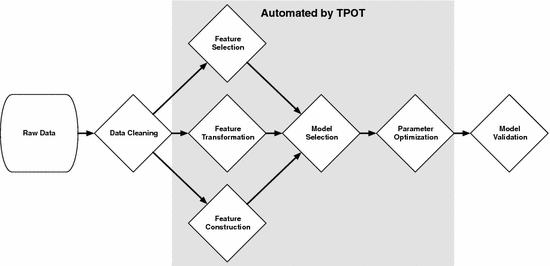
\includegraphics[width=1.0\columnwidth]{introduction/fig1h.png}
	\caption{Machine Learning Process using TPOT, \href{https://media.springernature.com/original/springer-static/image/chp\%3A10.1007\%2F978-3-319-31204-0_9/MediaObjects/419269_1_En_9_Fig1_HTML.gif}{source}}
\end{figure}

TPOT uses an evolutionary algorithm to automatically design and optimize a series of standard machine learning operations (i.e., a pipeline) that maximize the final classifier’s accuracy on a supervised classification dataset by using Genetic Algorithms and Pareto Optimization as depicted in Figure 2.2. 

\begin{figure}
	\centering
	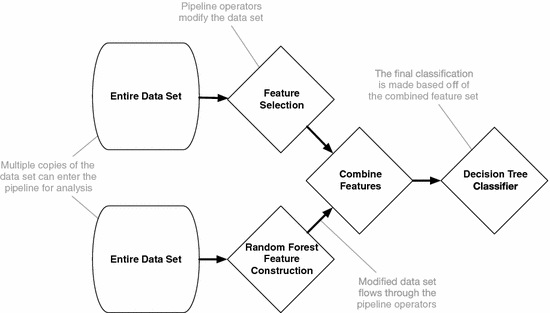
\includegraphics[width=1.0\columnwidth]{introduction/fig1i.png}
	\caption{TPOT, \href{https://media.springernature.com/original/springer-static/image/chp\%3A10.1007\%2F978-3-319-31204-0_9/MediaObjects/419269_1_En_9_Fig2_HTML.gif}{source}}
\end{figure}

\begin{figure}
	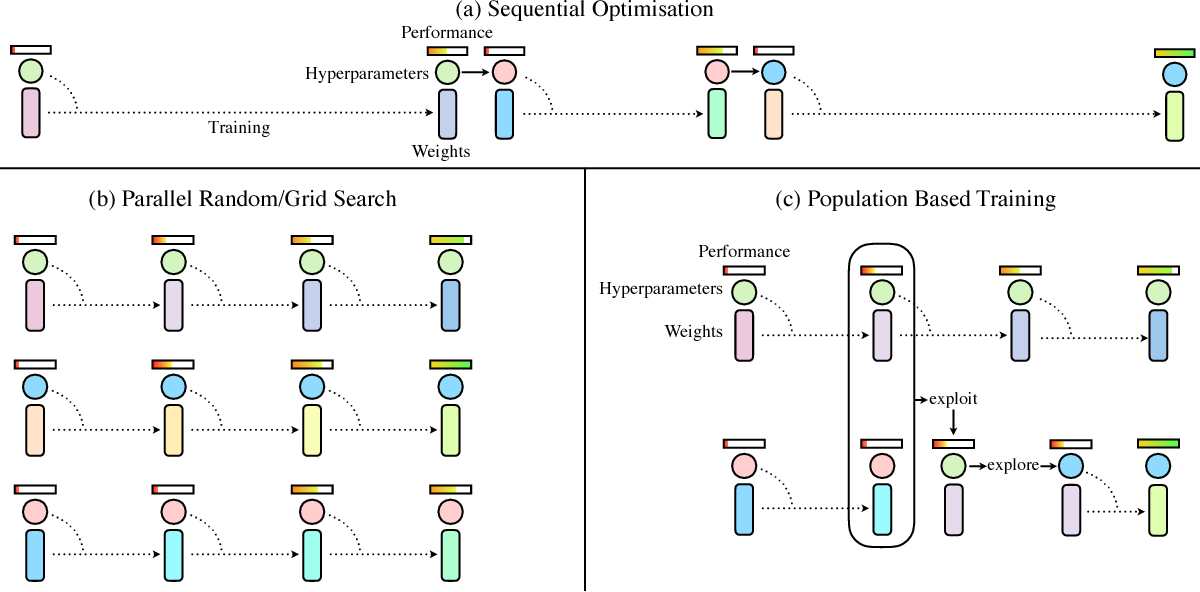
\includegraphics[width=1.0\columnwidth]{introduction/fig1j.png}
	\caption{Population Based Training of Neural Networks, \href{https://www.semanticscholar.org/paper/Population-Based-Training-of-Neural-Networks-Jaderberg-Dalibard/7a0b1f7fe39629360f1766a480dd8903065a2854/figure/0}{source}}
\end{figure}


\subsubsection{PBT}
In the seminal research on Neural Network training\cite{jaderberg2017population}, PBT or Population Based Training applies a hybrid model of random search and hand-tuning. Randomly initiated networks will be bred, trained and the hyper-parameters of the best performing network will be exploited by the rest of the networks. The process will continue till the number of generations are exhausted or the desired fitness of the network is achieved. 


\subsection{Quantum Inspired Genetic algorithm}
Due to seminal article showing polynomial run time of integer factorization\cite{shor1999polynomial}, researchers have been taking interest in emulating quantum computer on a classical machine. A result of which is Quantum Inspired Genetic Algorithm\cite{udrescu2006implementing}. 

Hybrid Genetic Algorithm (HGA)\cite{wang2005hybrid} is a GA that combines quantum operators (measure, quantum chromosomes, etc.) with classical genetic operators (crossover and mutation). HGA has been used for global optimization problems previously\cite{gonccalves2005hybrid}\cite{kim2007hybrid}\cite{kao2008hybrid}.



\subsection{Overview}
This section illustrated an overview of the emerging wisdom surrounding the development and the wide application base for Deep Neural Networks hyper-parameter optimization. The various methods by which Neural Networks are being adapted have been comprehensively discussed in this section. 

One issue that was completely overlooked in discussed implementations is the possibility of reaching local maxima instead of global maxima. Clearly this is a very important concern. Exploiting the hyper-parameters of the network with better accuracy, would impede the usage of hyper-parameters giving lower accuracy. This limits the possibility for achieving the best results.


\chapter{DESIGN}



\subsection{The framework}

The scope of this study is to access best set of hyper-parameters and train the neural network dataset. Previous section discussed software tools and algorithms that are currently in use by machine learning researchers. In this section, a panorama of the algorithm is discussed. The remaining sections, section 3.2, 3.3, 3.4 and 3.5 talk about the next stage of the panorama – design language and libraries, parallel computing and architectures.

\begin{figure}
	\centering
	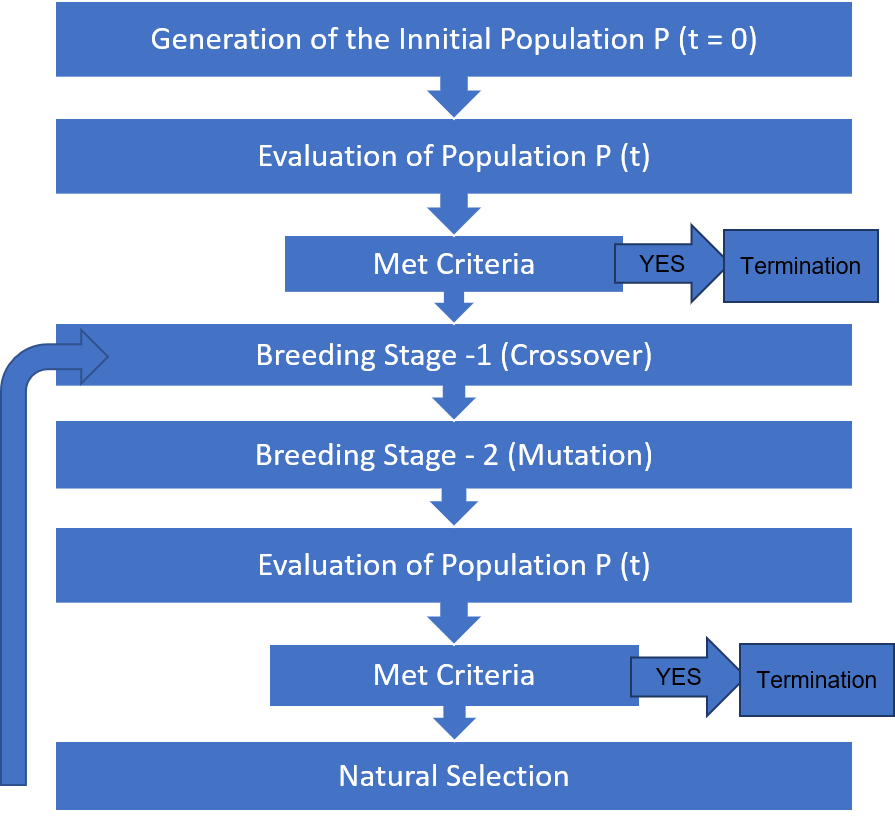
\includegraphics[width=1.0\columnwidth]{introduction/fig3a.png}
	\caption{Architecture Optimization Algorithm}
\end{figure}

\begin{figure}
	\centering
	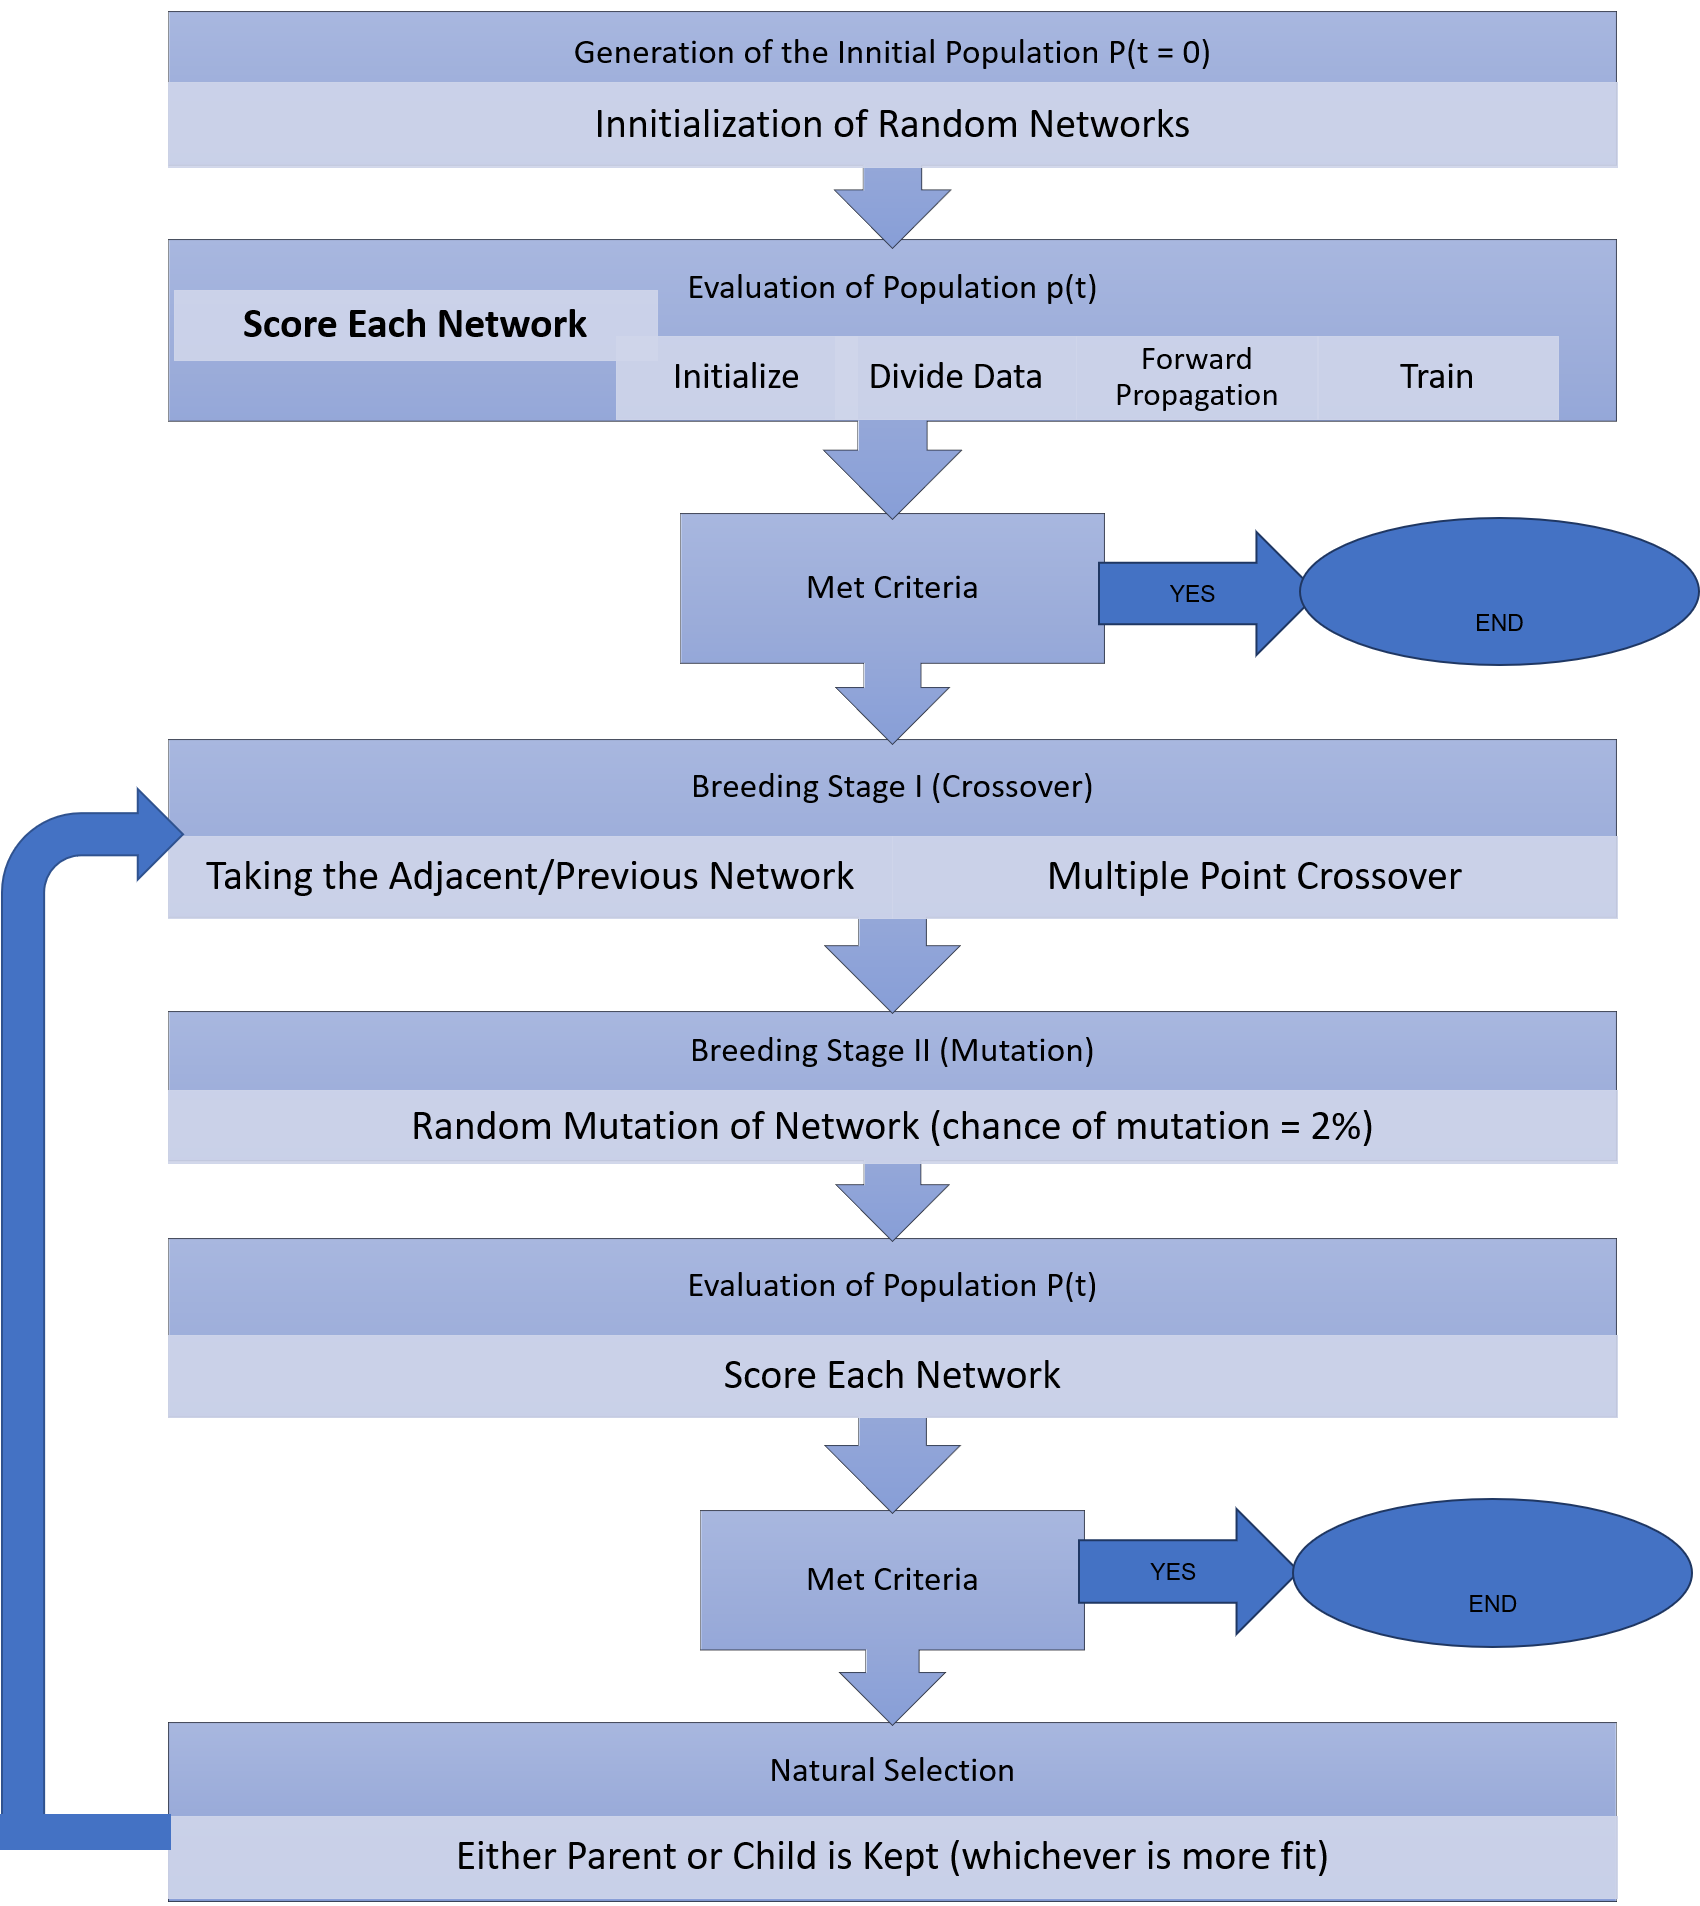
\includegraphics[width=1.0\columnwidth]{introduction/fig3b.png}
	\caption{Architecture for EETO for Neural Network Tuning}
\end{figure}

\begin{figure}
	\centering
	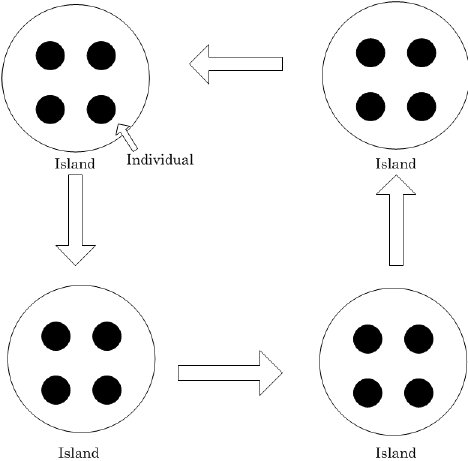
\includegraphics[width=0.5\columnwidth]{introduction/fig3c.jpg}
	\caption{Island Model, \href{https://www.researchgate.net/publication/284723071_Parallel_Genetic_Algorithms_on_a_GPU_to_Solve_the_Travelling_Salesman_Problem/figures?lo=1}{source}}
\end{figure}


The algorithm is designed to quickly get to the speed of neural network with the best possible accuracy; from first principles in Neural Network and Genetic Algorithm, all the way to discussions of some of the intricate details in Parallel Processing using MPI, with the purposes of achieving respectable performance on a machine learning benchmark: CIFAR10(classification of small images across 10 distinct classes: plane, car, bird, cat, deer, dog, frog, horse, ship and truck).


The model does so by selecting various hyper-parameters with different possible value combinations, followed by initiating the set of networks using those selected values and using the algorithm to crossbreed networks to compute the relative importance of parameter set to maximize the accuracy. 

With this, we will have acquired the fundamental structure of the model, to apply the algorithm to the interesting and difficult problem of fine tuning neural network parameters, with the trick of a parallelism to make it better than the initial baseline serial model (in terms of time and memory usage)

The architectures of the basic Optimization Algorithm - 'EETO' and the optimization algorithm 'EETO' for Neural Network Tuning are shown in Figure 3.1 and 3.2 respectively. A parallel implementation has also been applied which will be discussed in later section. Moreover, a parallel hybrid model -Island Model inspired by Island Model - Genetic algorithm is also implemented\cite{cantu1998survey}. The structure of the Island model is shown in Figure 3.3


\subsection{Software development}


Python comes with a very active user community and is overtaking in the race of popular programming languages. Even in HPC it has successfully found its way. With the advent of scientific python, python has become a successful contender\cite{insidehpc}. The language is not only clean, easy to implement but also comes with a vast number of open source libraries. The growing presence of libraries like cython, parallelpython(pp), Numba, Numpy, Mpi4py, makes python a reasonable choice for HPC. “Intel Parallel Studio XE 2017” Distribution for Python release claims to have shown a near native C performance with compilers and library packages optimized for the Intel architecture. Python libraries such as Numpy can make use of multithreading through calls to the Intel Threading Building Blocks (Intel TBB) library. Additionally, Intel Vtune provides line-by-line source code profiling to help find and correct issues causing performance hot spots or bottlenecks in Python source. 

In the race to be the fastest while PyPy has proven itself to be more than 500\% times faster than C version of python(CPython) \cite{pypy}, still there are algorithms where it is slower than equivalent code in C, involving a tradeoff between time and memory. For parts taking longer than average time, a python interface to C can be created, where data is passed from python and the routine is executed w/o any python overheads. These tools for easier interfacing include PySwip, pyrex and Cython. Although PySwip or Swi-Prolog offers a variety of development environment, multi-threading, comprehensive low-level interface to C, the memory usage of PySwip extensively using pointers slows down the system heavily. On the other hand, Pyrex which claims to be as fast as C language\cite{pyrexDocumentation}, comes with a bunch of limitations, as basic as not being able to access functions like local() and global()\cite{pyrexLimitations}. A more recent version - Cython compiler gives C-like performance along with Python bindings for many C and C++ libraries. But Cython is slowed down by Global Interpreter Lock (GIL). The lock keeps the Python virtual machine single-threaded, use of Python threads don't experience any concurrency unless I/O is involved (which frees the GIL). Fortunately, there are ways to overcome GIL mechanism viz. Multiprocessing and Mpi4py by offering a process-based parallelism using subprocesses instead of threads\cite{pythonDocumentation}.

 
Multiprocessors make use of shared memory, employ parallel processing techniques which limit their relevance to SMP-based hardware. However, Mpi4py would involve distributed memory. Mpi4py is cluster based and offers high scalability due to the relative absence of shared resources\cite{dalcin2008mpi}. As this thesis aims to exploit multiple nodes of a cluster, mpi4py is being used to leverage parallel computing. Since commands used from Mpi4py module support both mpirun and mpiexec, any of the Mpi execution can be used for running.


Next view of the “neural network” panorama, is the usage of Keras for Convolution Neural Network (CNN). Keras integrates with lower-level deep learning languages (in particular - TensorFlow) and has built-in support for multi-GPU data parallelism. Not only Keras use dozens of hyper-parameters, which are critical for the thesis, it comes with many datasets, models and layers, which can be imported into the code using simple import commands\cite{chollet2015keras}.


The complexity of these models could easily be extended beyond these capabilities to include any parameters included in Keras, allowing the creation of more complex architectures.



\subsubsection{Handling of SLURM workload manager}

Last but not the least, the codes are scheduled using SLURM workload manager.  SLURM comes with handy commands (view SLURM documentation using “man <command>”) each for scheduling, cancelling, viewing the status and possible starting time of jobs/nodes and managing usage of the node memory, accessing idle nodes, etc which are efficiently applied in this thesis. 
A refine built feature of this software is that depending on free window on a node, the code can be scheduled for the available time on that node and upon timeout, can be resumed (requires manual changes by the user in SLURM script and MAIN source file script) on another next available node. 


\subsection{Leveraging Parallel Computing}

Welcome to the third (and final) aspect in a series of designing of the algorithm. This section will, for the most part, assume familiarity with the previous two in the series.
Parallel computing is a type of computation in which many calculations or the execution of processes are carried out concurrently\cite{almasi1988highly}. With the industry-wide switch to multicore and manycore architectures, parallel computing has become the only venue in sight for continued growth in application performance\cite{hwu2014ahead}. Increasingly, parallel processing is being seen as a cost-effective method for the fast solution of computationally large and data-intensive problems\cite{kumar1994introduction}. Thus, the same has been applied in this thesis.


Parallel Algorithm primarily deals with dividing the networks into different processors to increase the efficiency of performing tasks and to reduce the time taken. However, various parallelization methods exist for dividing the populations to maximize efficiency. While implementing EETO parallelism In this thesis, analogy has been drawn from two major types of Parallel Genetic Algorithm (PGA): \textbf{Single-population fine-grained Genetic Algorithms}, and \textbf{Multiple-population Coarse-grained Genetic Algorithms}. These PGAs differ in terms of parallelization. A further description of these PGAs and the usage of each of the PGA is detailed below.

\begin{enumerate}

	\item Single Population Fine Grained Algorithms (SPFGA)
	Fine Grained Algorithm consists of multiple individuals evolving independently of each other. Each civilization consists of only one individual. Fine Grained Algorithm prevents premature convergence since each individual evolves independently. Further, this also provides the benefit of greater diversity. For these reasons, this type of algorithm supposedly outperforms all the other types of algorithms when dealing with high dimensional variable spaces\cite{li2007efficient}.
	Fine-grained PGA is more suitable for custom hardware design\cite{marakeby2013analysis}. Since each population has a single individual, a simple processor core is suitable for performing the tasks.
	
	\item Multiple-population Coarse Grained Algorithms (MPCGA)
	The coarse-grained (distributed) parallel algorithms assume the division of a large population into several subpopulations which are processed concurrently on different processing nodes\cite{wahib2011optimization}. They are also known as multi-deme GAs. Sub-populations evolve independently with only occasional exchange of individuals between them. Independent evolution allows for greater diversity and prevents premature convergence (similar to Fined Grained Populations).
	

\end{enumerate}
The architecture showing parallel implementation has been shown in Figure 3.4.


\begin{figure}
	\centering
	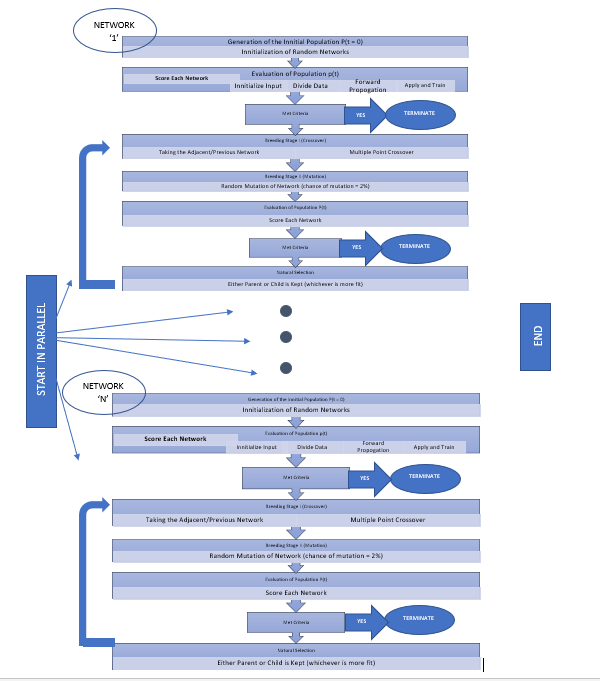
\includegraphics[width=1.0\columnwidth]{introduction/fig3d.png}
	\caption{Architecture for Parallel Neural Network Tuning}
\end{figure}




\section{HPC Cluster Architecture: Clusters, Installations}

\subsection{Development: Using Chuck Cluster}
The journey started with installations of softwares and libraries on chuck for development. Starting with python 3.7 which was not officially supported till 2018 June end, python 3.5 was the next version tried for this thesis, switching back and forth with python 2.7(supports best for tensorflow – dependency for Keras).


As discussed in the previous article, the main library used for neural networks training, i.e. keras was installed using pip3, which installed the latest version of keras(2.2.2). Since it used Tensorflow backend, the next challenge was to install Tensorflow. Tensorflow works on 64 bit systems. And the clusters’ architecture used in TCHPC are 64bit.
Somehow, the tensorflow latest version was throwing error: “Operation not permitted”, so switching to older version of tensorflow, i.e. tensorflow1.5 worked. Next step was to run the code, but that introduced to the next pitfall which was Binary incompatibility from numpy. Error:
“numpy.dtype size changed, may indicate binary incompatibility”
The solution is to check what packages depend on numpy and find out against what numpy version they were built. The error was a result of importing Keras that was compiled against a newer version of numpy than is installed.  Instead, installation of numpy1.14.5 worked. For that first the newer version of numpy is to be uninstalled and then the older version is to be installed. Now the binaries in the dependent packages are compatible. 


The summary of the steps is shown in the sequence graph in Figure 4.1.

\begin{figure}
	\centering%
	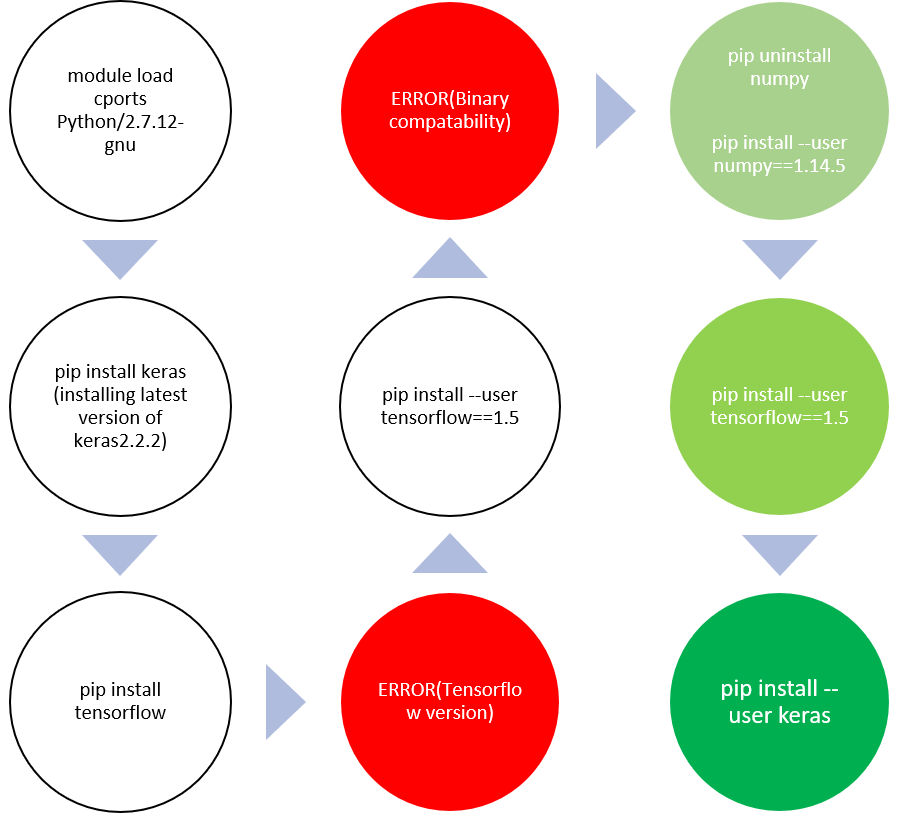
\includegraphics[width=0.8\columnwidth]{introduction/fig4a.png}
	\caption{Steps on TCHPC Chuck Cluster}
\end{figure}

All these installed adding '--user' at the end to install it in the home directory.

\subsection{Deployment Trial 1: Using Lonsdale Cluster}

The major problem faced was inability of getting Keras to work on Lonsdale or Kelvin. Following the steps taken while assessing the resources of the cluster Chuck, the tensorflow installation step threw error: 

\begin{verbatim}
    “/usr/lib64/libstdc++.so.6: version `GLIBCXX_3.4.14' not found”
\end{verbatim}

Digging further into the same showed, Chuck is on RHEL 7x and Lonsdale is on RHEL 6x. And it turns out that they have different GLIBC.  Default GLIBC on Lonsdale is 2.12. However, Tensorflow won’t work on anything except the absolute latest hardware. Tensorflow needs GLIBC >= 2.17
So, to be able to get Tensorflow on Lonsdale, the steps to be taken included:
\begin{enumerate}
	\item Installation of a new gcc version, 
	\item then compile bazel (a tool to compile tensorflow).
\end{enumerate}

\subsection{Deployment Trial 2: Using Kelvin Cluster}


The Kelvin Cluster has RHEL6.10 and the concern of GLIBC not supporting Tensorflow holds while using Kelvin Cluster. Solution to this would be to get to the cluster which has higher version Scientific Linux


\subsection{Deployment Trial 3: Using Boyle Cluster}

While there was a mismatch of the version and backend software requirements on Lonsdale and Kelvin, Boyle has the same Scientific Linux release as Chuck and thus, promises implementation of code. 

Lonsdale/ Kelvin:
\begin{enumerate}
	\item Scientific Linux release 6.10
	\item ldd (GNU libc) 2.12
\end{enumerate}


Boyle/ Chuck:
\begin{enumerate}
	\item Scientific Linux release 7.5 (Nitrogen)
	\item ldd (GNU libc) 2.17
\end{enumerate}

A brief of the HPC clusters\cite{TCHPC_clusters} is as follows: 

\begin{center}
	\begin{landscape}
	\begin{longtable}{||c c c c||}
		\hline
		Title & Boyle & Kelvin & Lonsdale \\ [0.5ex] 
		\hline\hline
		Server & Scientific Linux release 7.5 (Nitrogen) & Scientific Linux release 6.10 (Carbon) & Scientific Linux release 6.10 (Carbon) \\ 
		\hline
		Kernel Version & 3.10.0-862.3.3.el7.x86{\_}64 & 2.6.32-754.3.5.el6.x86{\_}64 & 2.6.32-754.3.5.el6.x86{\_}64 \\
		\hline
		GCC version & Red Hat 4.8.5 & Red Hat 4.4.7 & Red Hat 4.4.7 \\
		\hline
		Ldd Gnu LIBC & 2.17 & 2.12 & 2.12 \\
		\hline
		Processor Type & Intel & Intel & Opteron \\ 
		\hline
		RAM & 4.6TB & 2.4TB & 3.2TB \\
		\hline
		Interconnect & Mellanox ConnectX-3 QDR & Qlogic Infiniband QDR & Infiniband DDR \\
		\hline
		Theoretical Peak Performance & 43.378TF & 12.76TF & 11.33TF \\
		\hline
		Linpack Score & 33.536TF &   & 8.9TF \\
		\hline
		Number of Nodes & 33 & 100 & 154 \\
		\hline
		ArchitecturE & 64 & 64 & 64 \\
		\hline
		Ram/node & 64 & 24 & 16 \\
		\hline
		RAM & 4.6TB & 2.4TB & 3.2TB \\
		\hline
		Num cores & 804 & 1200 & 1243 \\
		\hline
		Number of sockets/node & 2 & 2 & 2 \\
		\hline
		Number of cores per socket & 8 & 6 & 4 \\
		\hline
		Clock Speed & 2.00GHz & 2.66GHz & 2.30GHz \\
		\hline
		Available to & Selected Groups & Irish Researchers & TCD Researchers \\ [1ex] 
		\hline
	\end{longtable}
	\end{landscape}
\end{center}

Side-stepping re-installations of any library and preservation of the work done on compatibility testing of libraries, one of the four tools viz. Virtualenv, Native pip, Docker, or Anaconda can be used. This thesis makes use of Anaconda. Anaconda or conda is a mechanism to keep the dependencies required by different projects in separate places, making it reliable and easy for using various libraries. Conda installs TensorFlow and all the required and/or dependent packages. Activating the environment will activate all the packages installed in that environment. The environment packages can be viewed using “conda list”. 
Installing TensorFlow with pip in a conda environment may cause issues. The conda installation would take precendent over the pip installation. This means that after importing tensorflow in python, “tensorflow.{\_}{\_}version{\_}{\_}” would return the version installed through conda.
Last but not the least is installation of Mpi4py, which can be installed using conda install command.



Recap of configurations:


\setlength\parindent{24pt} Server: Scientific Linux release 7.5 (Nitrogen)

\setlength\parindent{24pt} conda 4.5.10

\setlength\parindent{24pt} Python 2.7.15 :: Anaconda, Inc.

\setlength\parindent{24pt} numpy 1.15.0

\setlength\parindent{24pt} Keras 2.2.2

\setlength\parindent{24pt} Tensorflow 1.5

\setlength\parindent{24pt} Mpi4py 2.0.0

\setlength\parindent{24pt} gcc: gcc (GCC) 4.8.5 20150623 (Red Hat 4.8.5-28)

\setlength\parindent{24pt} ld: ldd (GNU libc) 2.17


\section{Installation steps}

See Figure 4.2 for a detailed introduction of how the installation and code works and some basic usage.

\begin{figure}
	\centering
	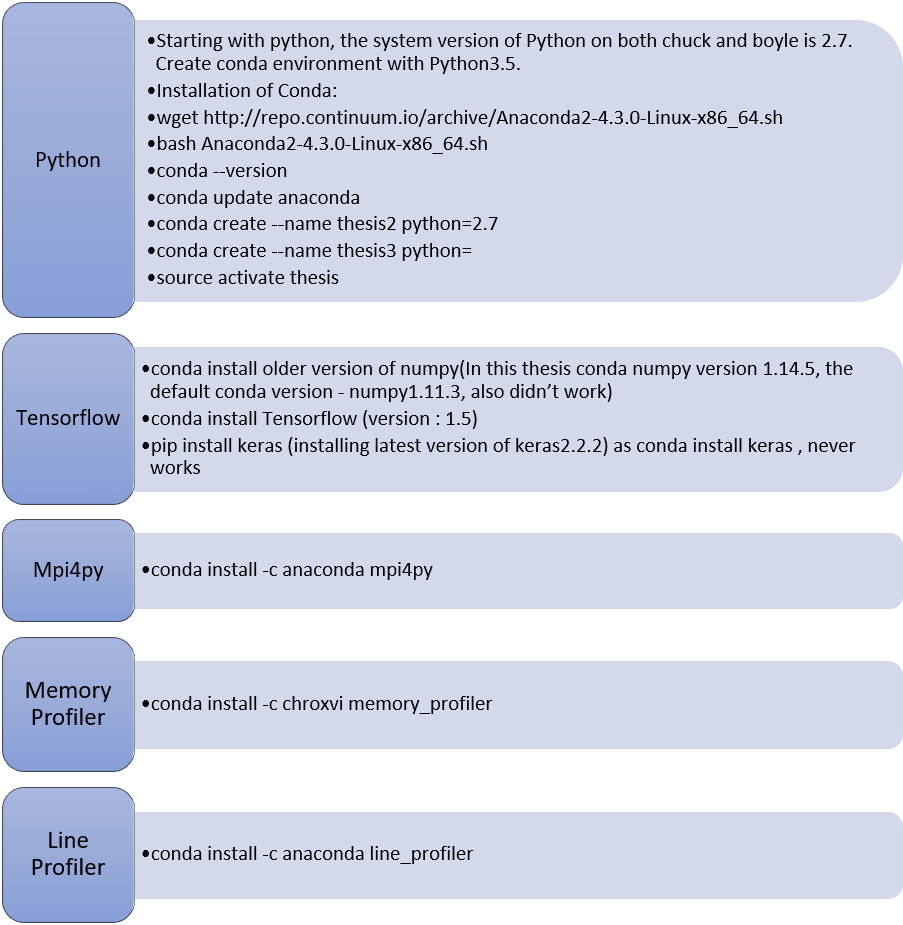
\includegraphics[width=1.0\columnwidth]{introduction/fig4b.png}
	\caption{Steps to install libraries}
\end{figure}

\section{Introduction to the code for Simulation }

The sections explains the pseudo code for the various algorithms used.


\textbf{Pseudo Codes Neural Network Tuning - NNT}

\begin{enumerate}
	\item start
	\begin{enumerate}
		\item Initialize Input
		\item Define Input data
		\item Define output data
	\end{enumerate}
	\item Divide data into training and test data
	\begin{enumerate}
		\item In this Thesis, Cifar10 dataset is considered, with total 60k data points
		\item test data = 10k data points (~ 15%)
		\item Training data=50k data points (~ 85%)
	\end{enumerate}
	\item Define layers, neuron units in each layer, activation function, optimizer and dropout
	\item Fit the model
	\begin{enumerate}
		\item Feed Forward neural Network
	\end{enumerate}
	\item Compile the model
	\item Make total error = 0
	\item Train the neural network
	\item Evaluate the fitness of the network
	\item Total error += Error for each output neuron
	\item If total error < target error => Terminate, else
	\begin{enumerate}
		\item Continue Step 6
	\end{enumerate}	
\end{enumerate}


\textbf{Pseudo Codes Sequential Algorithmic for Neural Network Tuning}
\begin{enumerate}
	\item Initialize population or network
	\item Train each network
	\item Evaluate the fitness of each network
	\item Check the criteria
	\begin{enumerate}
		\item number of generations
		\item Fitness achieved
	\end{enumerate}
	\item If achieved then terminate, else
	\begin{enumerate}
		\item Breed Networks
		\item Train each network
		\item Evaluate fitness of each network
		\item Select the best networks for next generations
		\item Continue Step 4
	\end{enumerate}
\end{enumerate}



\textbf{Pseudo Codes Parallel Algorithm for Neural Network Tuning}

\begin{enumerate}
	
	\item Initialize population or network (one per processor)
	\item Train network on each processor
	\item Evaluate the fitness of each network on the processors
	\item Check the criteria
	\begin{enumerate}
		\item number of generations
		\item Fitness achieved
	\end{enumerate}
	\item If achieved then terminate, else
	\begin{enumerate}
		\item Breed Networks
		\begin{enumerate}
			\item Crossover (take network from previous processor for crossover)
			\item Mutation (Chance of mutation is considered 2%)
		\end{enumerate}
		\item Train each network
		\item Evaluate fitness of each network
		\item Select the best networks for next generations
		\item Continue Step 4
	\end{enumerate}
\end{enumerate}


\textbf{Pseudo Codes Parallel Island Model based Algorithm for Neural Network Tuning}

\begin{enumerate}
	
	\item Initialize islands
	\item Initialize island population 
	\item Train island networks 
	\item Evaluate the fitness of each network on the processors
	\item Check the criteria
	\begin{enumerate}
		\item number of generations
		\item Fitness achieved
	\end{enumerate}
	\item If achieved then terminate, else
	\begin{enumerate}
		\item Breed Networks
		\begin{enumerate}
			\item Crossover (take network from previous processor within the island for crossover)
			\item Mutation (Chance of mutation is considered 2%)
		\end{enumerate}
		\item Train each network
		\item Evaluate fitness of each network
		\item Select the best intra-island network for next generations
		\item Continue Step 4
	\end{enumerate}
	\item If generation number is a multiple of 10, then
	\begin{enumerate}
		\item Breed Networks
		\begin{enumerate}
			\item Inter-island Crossover 
			\item Mutation (Chance of mutation is considered 2%)
		\end{enumerate}
		\item Train each network
		\item Evaluate fitness of each network
		\item Select the best networks for next generations
		\item Continue Step 4
	\end{enumerate}
\end{enumerate}



\textbf{Pseudo Codes for Quantum Inspired Algorithm for Neural Network Tuning}

\begin{enumerate}
	\item Initialize quantum population vector Q
	\item Train each network in the Q vector
	\item Evaluate the fitness of each network in the Q vector
	\item Check the criteria
	\begin{enumerate}
		\item number of generations
		\item Fitness achieved
	\end{enumerate}
	\item If achieved then terminate, else
	\begin{enumerate}
		\item Breed Networks (Quantum Crossover using superposition)
		\item Train each network
		\item Evaluate fitness of each network
		\item Select the best networks for next generations
		\item Continue Step 4
	\end{enumerate}
\end{enumerate}


\textbf{Github Code repository Links:}

\href{https://github.com/bhatnags/NeuralNetworkOptimization_EETO}{Neural Network Optimization Github Repository}




\section{Sequential Concern}

\subsubsection{SSE Speed Limitations}
Careful observation in the output file suggests that if TensorFlow is built from source it can be faster on the machine. The error is as follows:
“The TensorFlow library wasn't compiled to use SSE instructions, but these are available on your machine and could speed up CPU computations”
And it requires bazel build, which has gcc build constraints 


\subsubsection{Training Speed Constraint}
In this thesis, optimization of Neural Network parameters requires faster computation of the evaluation function. Since with generations during optimization, multiple populations are evaluated and replaced on a generational basis, the algorithm poses memory and time constraints. As we have seen in the above cluster comparison, Boyle has limited nodes and using only one OMP THREAD drags the whole training process of one genome to an hour.
If one evaluation takes 1 hour, then for over 1000 population, evaluations can be deadening to the cluster. In this thesis, generations are constrained to the limit of 30




\chapter{IMPLEMENTATION AND DATA ANALYSIS}

Exploration vs Exploitation based Optimization (EETO) Method has been implemented in Sequential Code. The same has been parallelized using Mpi4py. Next, the population initialization method of EETO has been inspired using concepts of Quantum Mechanics. The implementation is discussed in detail in below subsections.

In all the methods, the search space has been kept constant. A group of 5 hyper-parameters has been considered:
activation functions, optimizers, hidden layers, nodes in hidden layers
and dropout. Six activation functions included are: sigmoid, elu, selu, relu, tanh, hard\_sigmoid. In addition to this, optimizers include sgd, adagrad, adadelta, adam, adamax, nadam. Hidden layers range from 1-15. Nodes/neurons range from 4-128. Dropouts range from 0.1 to 0.5.

In all the methods, the networks are initialized using random sets
of configuration variables. These networks then exchange
hyper-parameters with each others(exploitation). The networks get
the change to mutate @30\%. This process is called as breeding. Based on fitness values, the network with least fitness value is killed/deleted and re-initialized (Exploration). 


\section{Genetics Inspired Exploration vs Exploitation based Optimization for Neural Network Tuning}

\subsection{Implementation}

Several implementations of the same have been done using different number of processes (5 implementation using network size of 4, 6, 8, 10, 12 respectively)

\textbf{Requirements:}
\begin{enumerate}
	\def\labelenumi{\arabic{enumi}.}
	%\tightlist
	\item
	Server: Scientific Linux release 7.5 (Nitrogen)
	\item
	conda 4.5.10
	\item
	Python 2.7.15 :: Anaconda, Inc.
	\item
	numpy 1.15.0
	\item
	Keras 2.2.2
	\item
	Tensorflow 1.5
	\item
	gcc: gcc (GCC) 4.8.5 20150623 (Red Hat 4.8.5-28)
	\item
	ld: ldd (GNU libc) 2.17
\end{enumerate}

\textbf{Usage:}

\begin{verbatim}
python snnt.py
\end{verbatim}

This saves the output in a log file.

\subsection{Analysis}

The fitness values for various hyper-parameters are analyzed

Number of networks initialized = 4, Processors used = 1

A crossstab of the tested combinations of hyper-parameters is
shown below. It can be easily seen from Figure 4.1 that while evaluating hyper-parameter
combinations for training out of 6 activation functions, 'hard\_sigmoid'
and 'elu' could not be tested with optimizer 'adagrad', implying that not all the functions could be tested

\begin{figure}
	 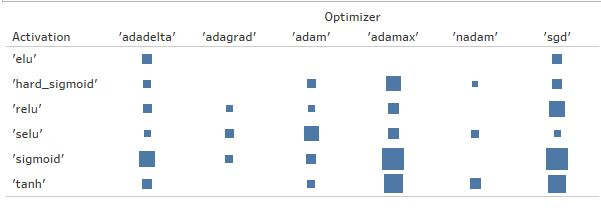
\includegraphics[width=\textwidth]{../../EETO/ResultAnalysis/optimizerVSActivation.jpg}
	 \caption{Cross tab of activation functions and optimizers tested }
\end{figure}

Next, a heat map of hyper-parameters' set and the fitness thusly achieved has been created as shown in Figure 4.2. From this it can be concluded that fitness is highly related to the number of neurons.

\begin{figure}
	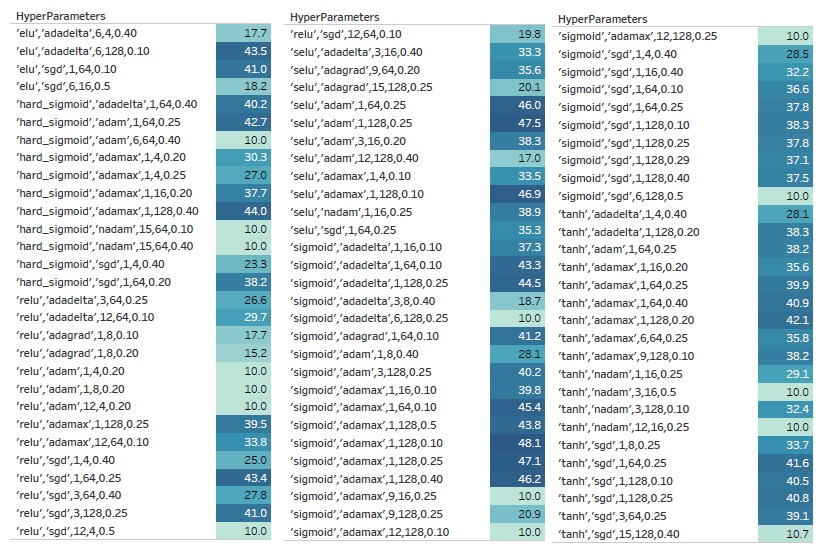
\includegraphics[width=1.1\textwidth]{../../EETO/ResultAnalysis/4s.jpg}
	\caption{Sampled hyper-parameters' set; \newline Column 1 (from Left to Right): Activation function, Optimizer, Layers, Neurons, Dropout; \newline Column 2: Maximum Fitness for the hyper-parameter combination;}
\end{figure}

A more detailed plot is as follows (Figure 4.3). The size of the squares denote the
fitness. While increment in number of neurons increase the fitness, decrement in number of layers help improvise the fitness.

\begin{figure}
	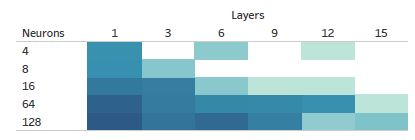
\includegraphics[width=\textwidth]{../../EETO/ResultAnalysis/neuronsVSlayers.jpg}
	\caption{Fitness Heat Map - neurons va layers}
\end{figure}


With 4 random networks initialization of best combination of hyper-parameters is highly unlikely, since total possible combinations of hyper-parameters is tens of thousands.
However, if with the help of HPC, speed could be achieved then the same could be run for thousands of generations and with higher number of networks increasing the possibility of a better accuracy network. To test the same, networks of size 6, 8, 10 and 12 have been run in sequential and parallel. The next section discussed the effectiveness of the same.


\section{PGA Inspired Exploration vs Exploitation based Optimization for Neural Network Tuning}



\subsection{Implementation}

As discussed in the previous section, two parallel software implementations of the algorithm are employed for development. Keeping everything constant, the implementations differ in the arrangement of the networks. Exploring the same space, both the implementations use Mpi4py for parallelism. Since the networks being evaluated at processors are not equal in size, MPI Barrier is used.



\begin{enumerate}
	\item In Single Population Fine Grained Algorithms (SPFGA), the serial code is run using multiple processors. Every processor initiates one network. For crossover, network of the previous rank is taken. The bred child is mutated considering 30\% mutation chance. In this analysis, multiple codes are run using 4, 6, 8, 10, 12 processors.
	
	
	In this method, a send and receive model of GA is used. For each node, one network is initiated. Assuming more nodes ensures increased input combinations, will result in increased possibility of getting desired accuracy in the initial stages. Safety flags like are used to ensure MPI initialization has been successful. Breeding of one child per processor occurs. Considering processors structured in circular fashion, Crossover takes network from previous processor using MPI Non-Blocking Communication.
	\item Multiple-population Coarse Grained Algorithms (MPCGA) model uses the same concept as stated above. However, multiples island are initialized with population in each island. Two types of breeding takes place, inter-island(after every 5 generations) and intra-island. In this, population size of 4 in each island with 3 islands and total of 12 processes is run. Multiple islands of population are created viz. multiple MPI communicators for sets of networks are created. 
	
	
	Using the same hypothesis as previously used, “assuming more nodes ensures increased input combinations, will result in increased possibility of getting desired accuracy in the initial stages”, for each node, one network is initiated. These networks are then split into communicators. Breeding of one child per processor occurs, however crossover is intra-communicator, implying that same circular fashion of processors for every communicator is assumed and the processors are mated with the previous processors.
	After every “x”(in this thesis, x is kept 5) number of generations, inter-communicator crossover occurs in which best of every communicator/island is computed at every node using MPI gather and MPI scatter commands and is sent to the other islands. This process continues till either required accuracy is achieved or the limit for the number of generations have been crossed.
	
\end{enumerate}


\textbf{Requirements:}

\begin{enumerate}
	\def\labelenumi{\arabic{enumi}.}
	%\tightlist
	\item
	Server: Scientific Linux release 7.5 (Nitrogen)
	\item
	conda 4.5.10
	\item
	Python 2.7.15 :: Anaconda, Inc.
	\item
	numpy 1.15.0
	\item
	Keras 2.2.2
	\item
	Tensorflow 1.5
	\item
	gcc: gcc (GCC) 4.8.5 20150623 (Red Hat 4.8.5-28)
	\item
	ld: ldd (GNU libc) 2.17
	\item
	Mpi4py 2.0.0
\end{enumerate}

\textbf{Usage:}

\begin{verbatim}
mpiexec -n 7 python dnnt.py
mpiexec -n 7 python innt.py
\end{verbatim}

This saves the output in log files. The code can be run in accordance with the availability of cluster nodes



\subsection{Comparative Analysis}


A comparison of fitness evolution with generations is drawn for various ranks as shown below.
Starting with analysis on code using 4 networks initialized on 4
processors in parallel. The below image (Figure 4.4) shows that there is very slight difference in the fitness between two methods.
Figure 4.4 shows the fitness achieved by various implementations.
The graphs in the left hand side are for sequential method, the graphs in the right hand side are the parallel method. Both the methods are run for various network sizes (4, 6, 8, 10, 12). The graph shows the line chart for fitness conversion with respect to the number of generations passed. In both sequential and parallel implementations, the fitnesses are converging to a value of 50\%
However, the accuracy that serial code taken hours to achieve can be gained in minutes time running parallel code.



This shows that increasing the number of ranks/networks has no impact on
fitness, however, increasing the ranks for the analysis does help in
getting the fitness sooner.


\begin{figure}
	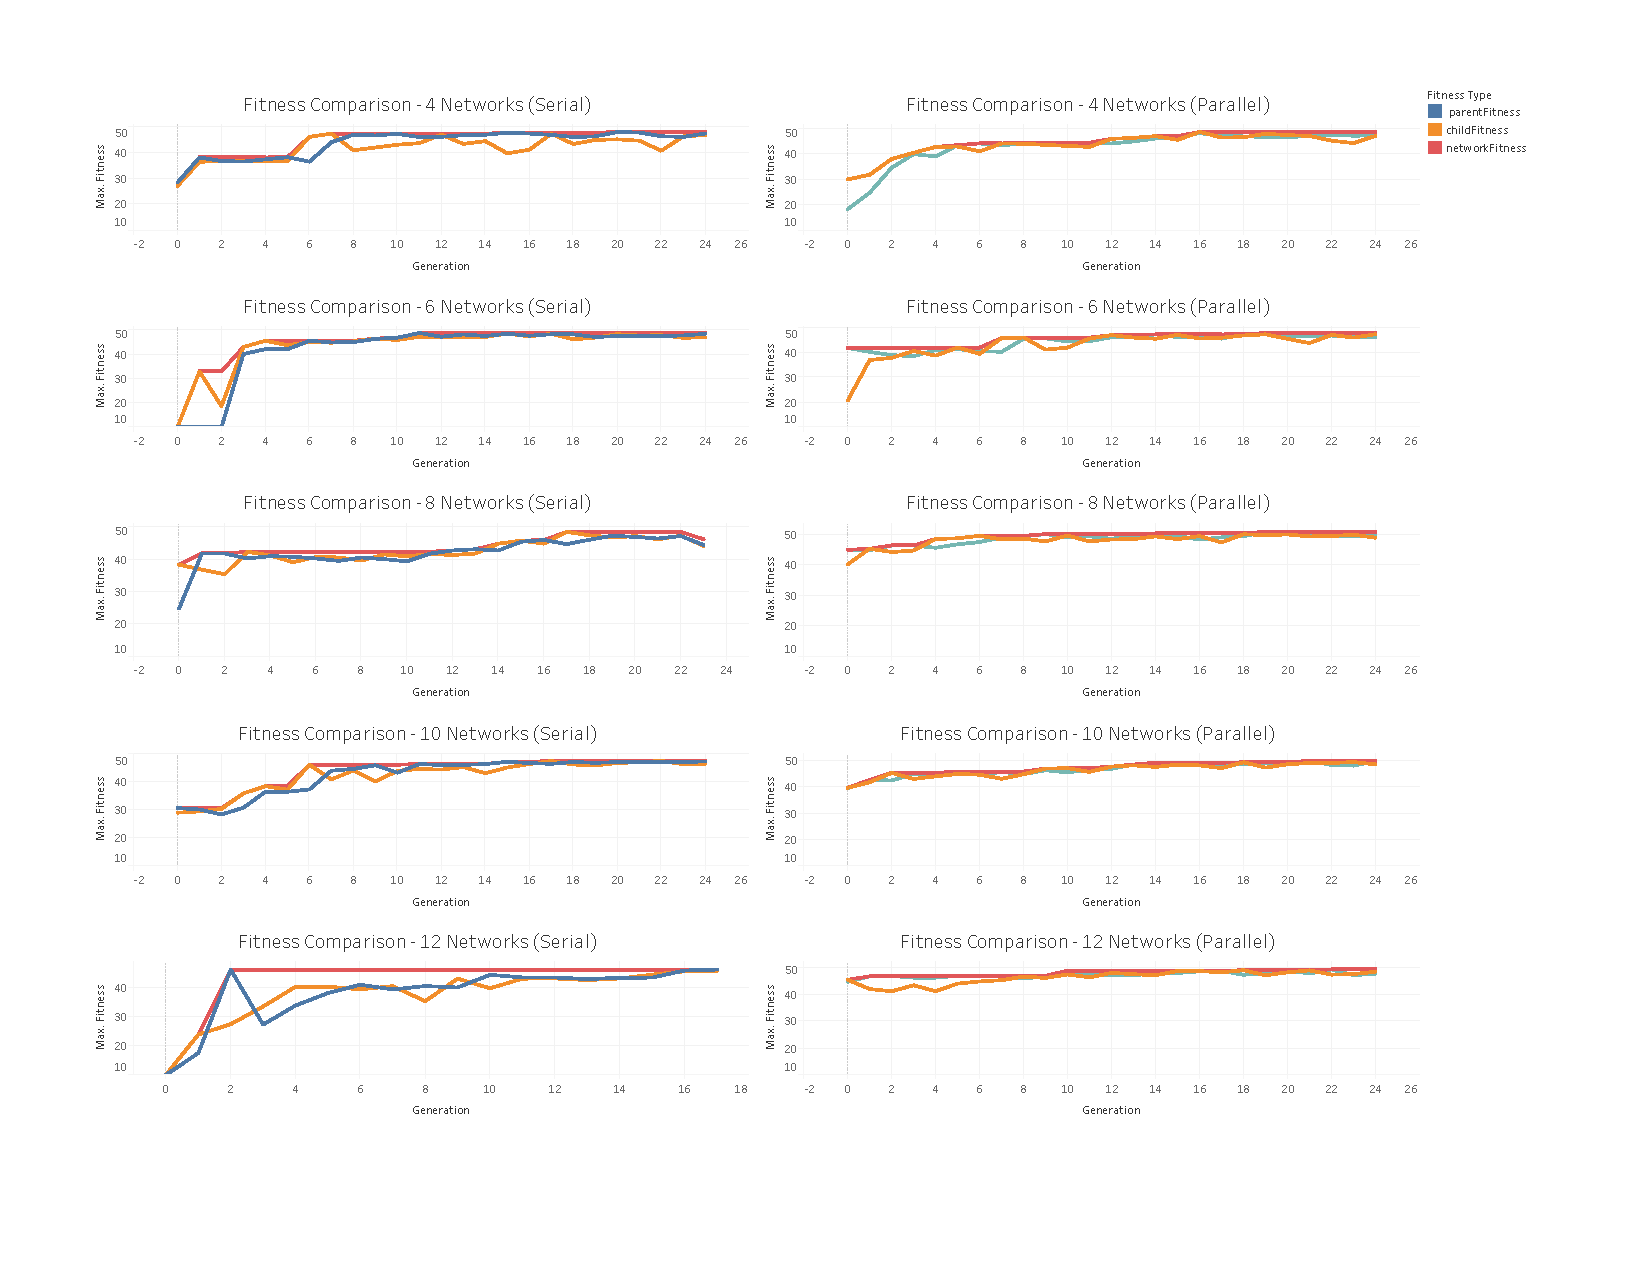
\includegraphics[height=0.62\textheight]{../../EETO/ResultAnalysis/FitnessComparison.pdf}
	\caption{Fitness comparison - Sequential vs Parallel Implementation;\newline Left Hand Side: Fitness results for Sequential Implementation with different network sizes;\newline Right Hand Side: Fitness results for Parallel Implementation with different network sizes;
	\newline Top to bottom: Fitness evaluation graphs for Network sizes 4, 6, 8, 10, 12;
	\newline Fitness are being captured at generation level;}
\end{figure}

\begin{figure}
	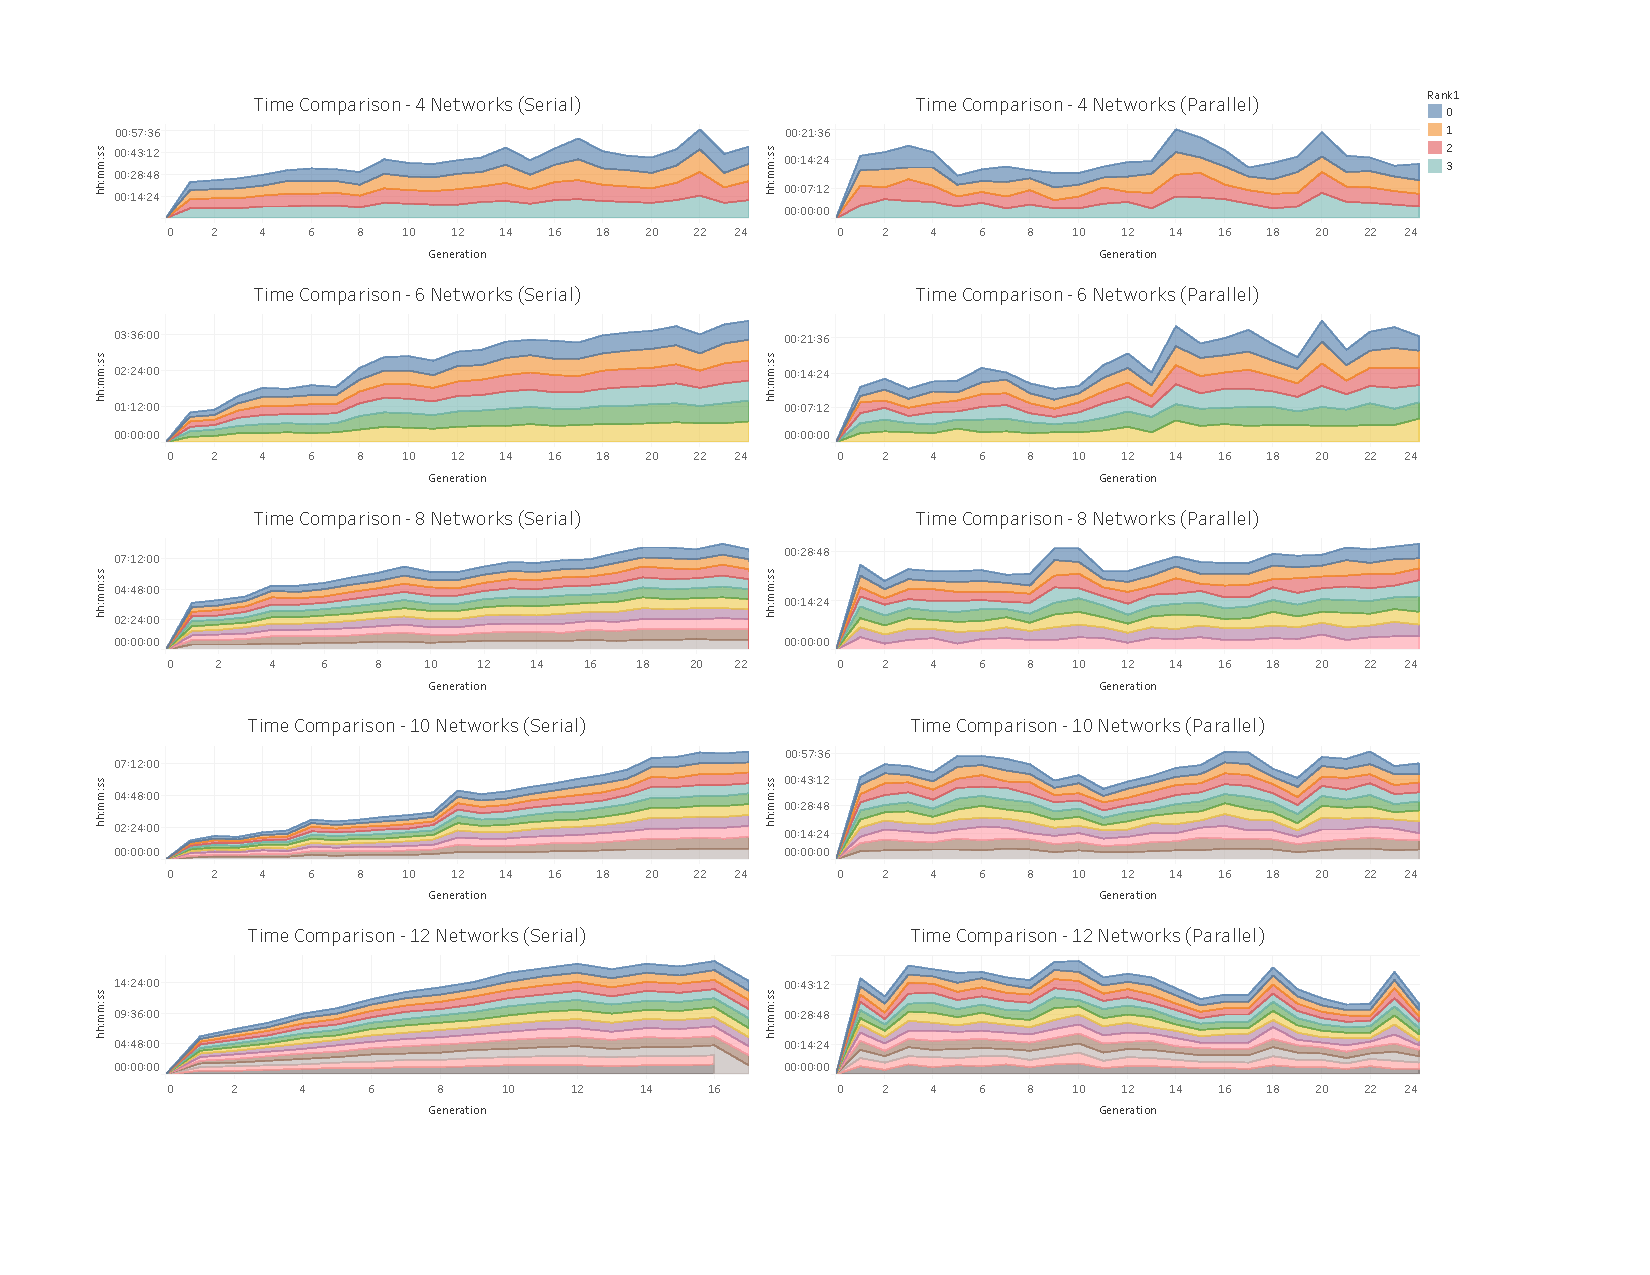
\includegraphics[height=0.65\textheight]{../../EETO/ResultAnalysis/TimeComparison.pdf}
	\caption{Time comparison - Sequential vs Parallel Implementation\newline Left Hand Side: Results for time taken in Sequential Implementation with different network sizes;\newline Right Hand Side: Results for time taken in Parallel Implementation with different network sizes;
	\newline Top to bottom: Graph depicting Time Taken for Network sizes 4, 6, 8, 10, 12;
	\newline Area graph for Time taken is shown at generation level;}
\end{figure}


Figure 4.5 shows the area graph of the time taken by various implementations. The presentation follows the same structure as the fitness graph in Figure 4.4.
Comparing the same with graphs plotted for the serial implementation, it can be easily concluded that
time taken to train each network in parallel is less than the time taken
while training in sequential. The reason behind such behavior is
division and ease of access of RAM for each network. Keras add sessions everytime a model is trained.
The reduction of time at generation level is due to division of tasks in parallel reducing the amount of time taken as per ``Law of division of labor''


In sequential graph, the time taken increases with generations.
In the beginning it was believed that this is due to memory constraints as the python library that is used for optimization "keras", saves the models and the hyper-parameters, parameters and other required variables for further cross-checking.


\subsubsection{Island Model}


The same is tested creating Island model.
Three islands of size 4 each have been created. Below is the graph (Figure 4.6) at generation level, comparing the time taken by the Island model implementation vs the time taken by the sequential and the parallel implementations to achieve the same fitness.
One of the Islands Island group 0 out of the three Islands (Island Group 0, 1 and 2) have been plotted against Sequential and parallel with network size of 4 each.


\begin{figure}
	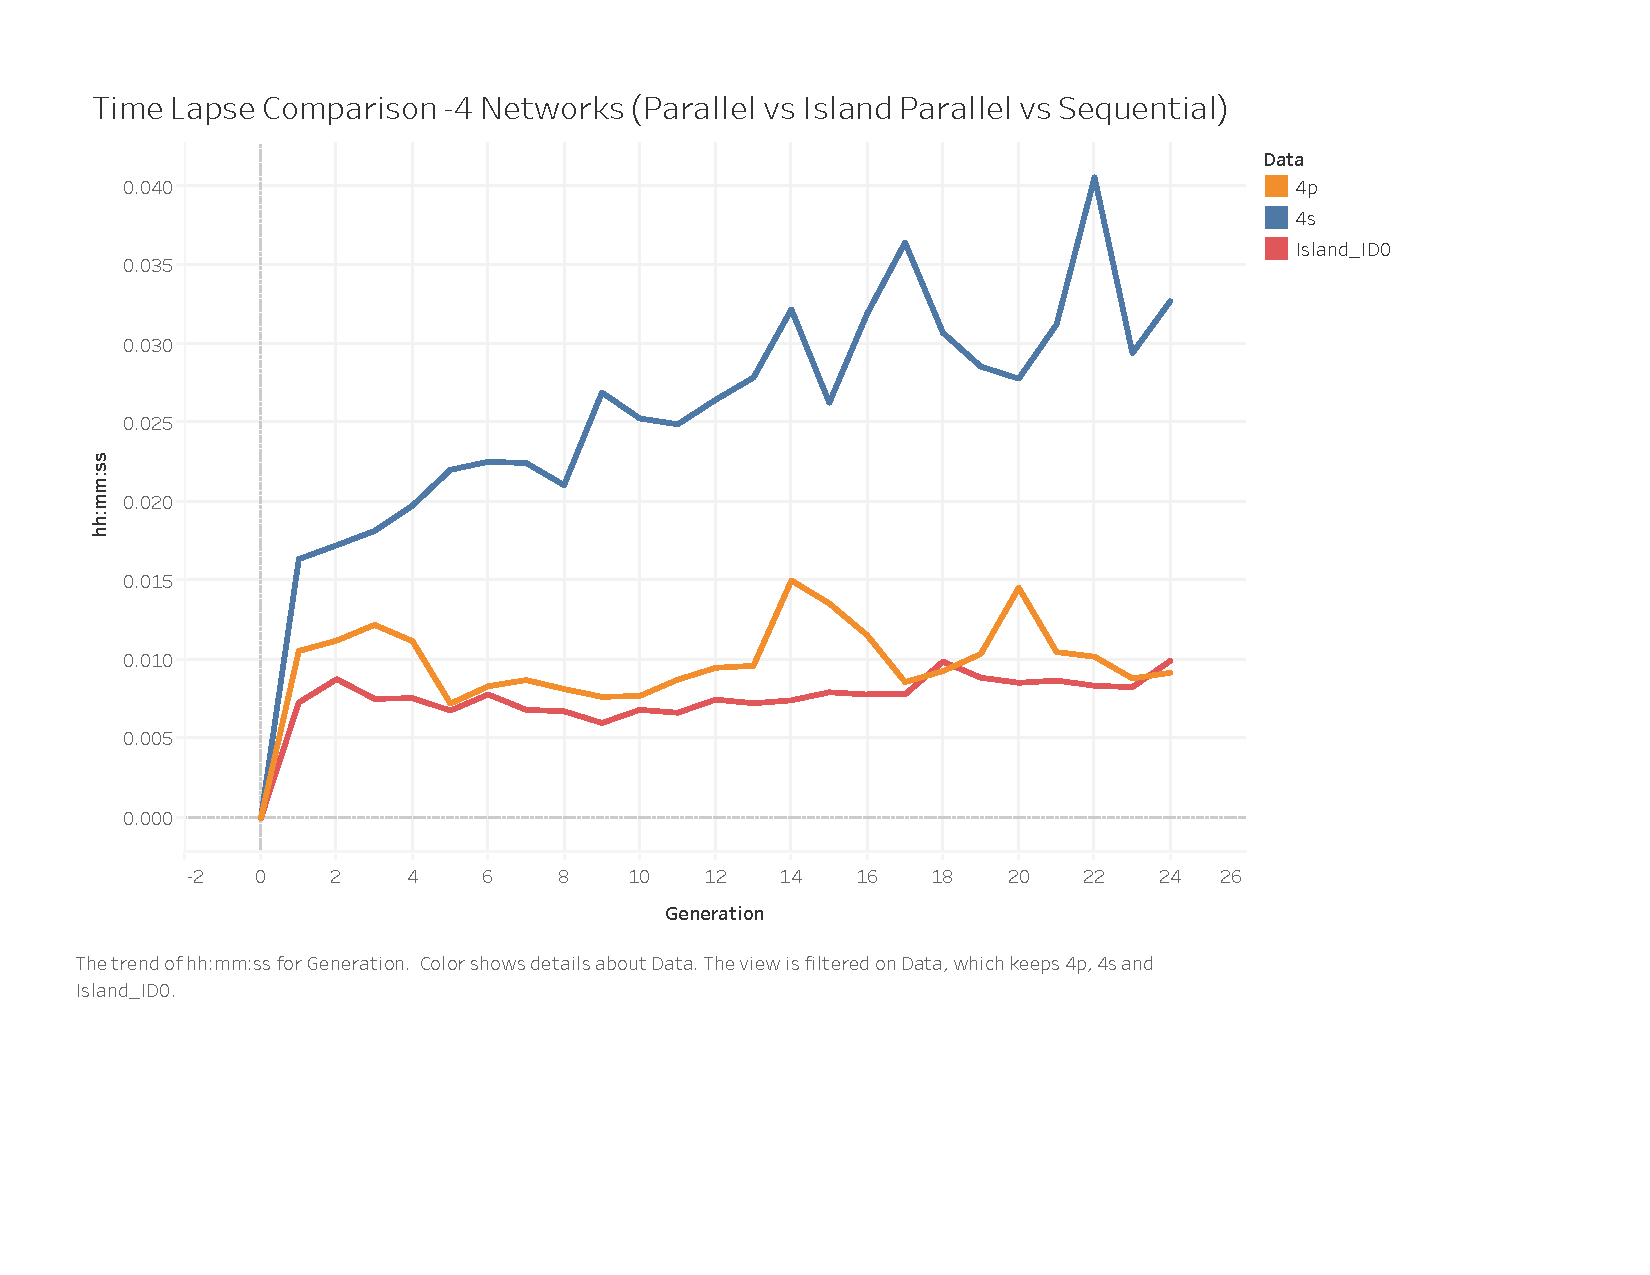
\includegraphics[height=0.68\textheight]{../../EETO/ResultAnalysis/TimeLapseIsland.pdf}
	\caption{Time comparison - Sequential vs Parallel vs Island Implementation; \newline Legend Decode: \newline \textbf{4s} -> 4 Networks Genetics Inspired Algorithm Data; \newline  \textbf{4p} -> 4 Networks Parallel Algorithm Data; \newline  \textbf{Island\_ID0} -> 4 Networks Genetic Algorithm Island Algorithm Data using only one Island group with ID "0"}
\end{figure}



From the above table it can be inferred that implementation of the island model resulted is fruitful in terms of time taken.

However, the graph of the sequential implementation is alarming as the time taken is increasing with generations.

\textbf{Memory Limits}

Furthermore, the efficiency and speed-up graphs are plotted as shown in Figure 4.7.

\begin{figure}
	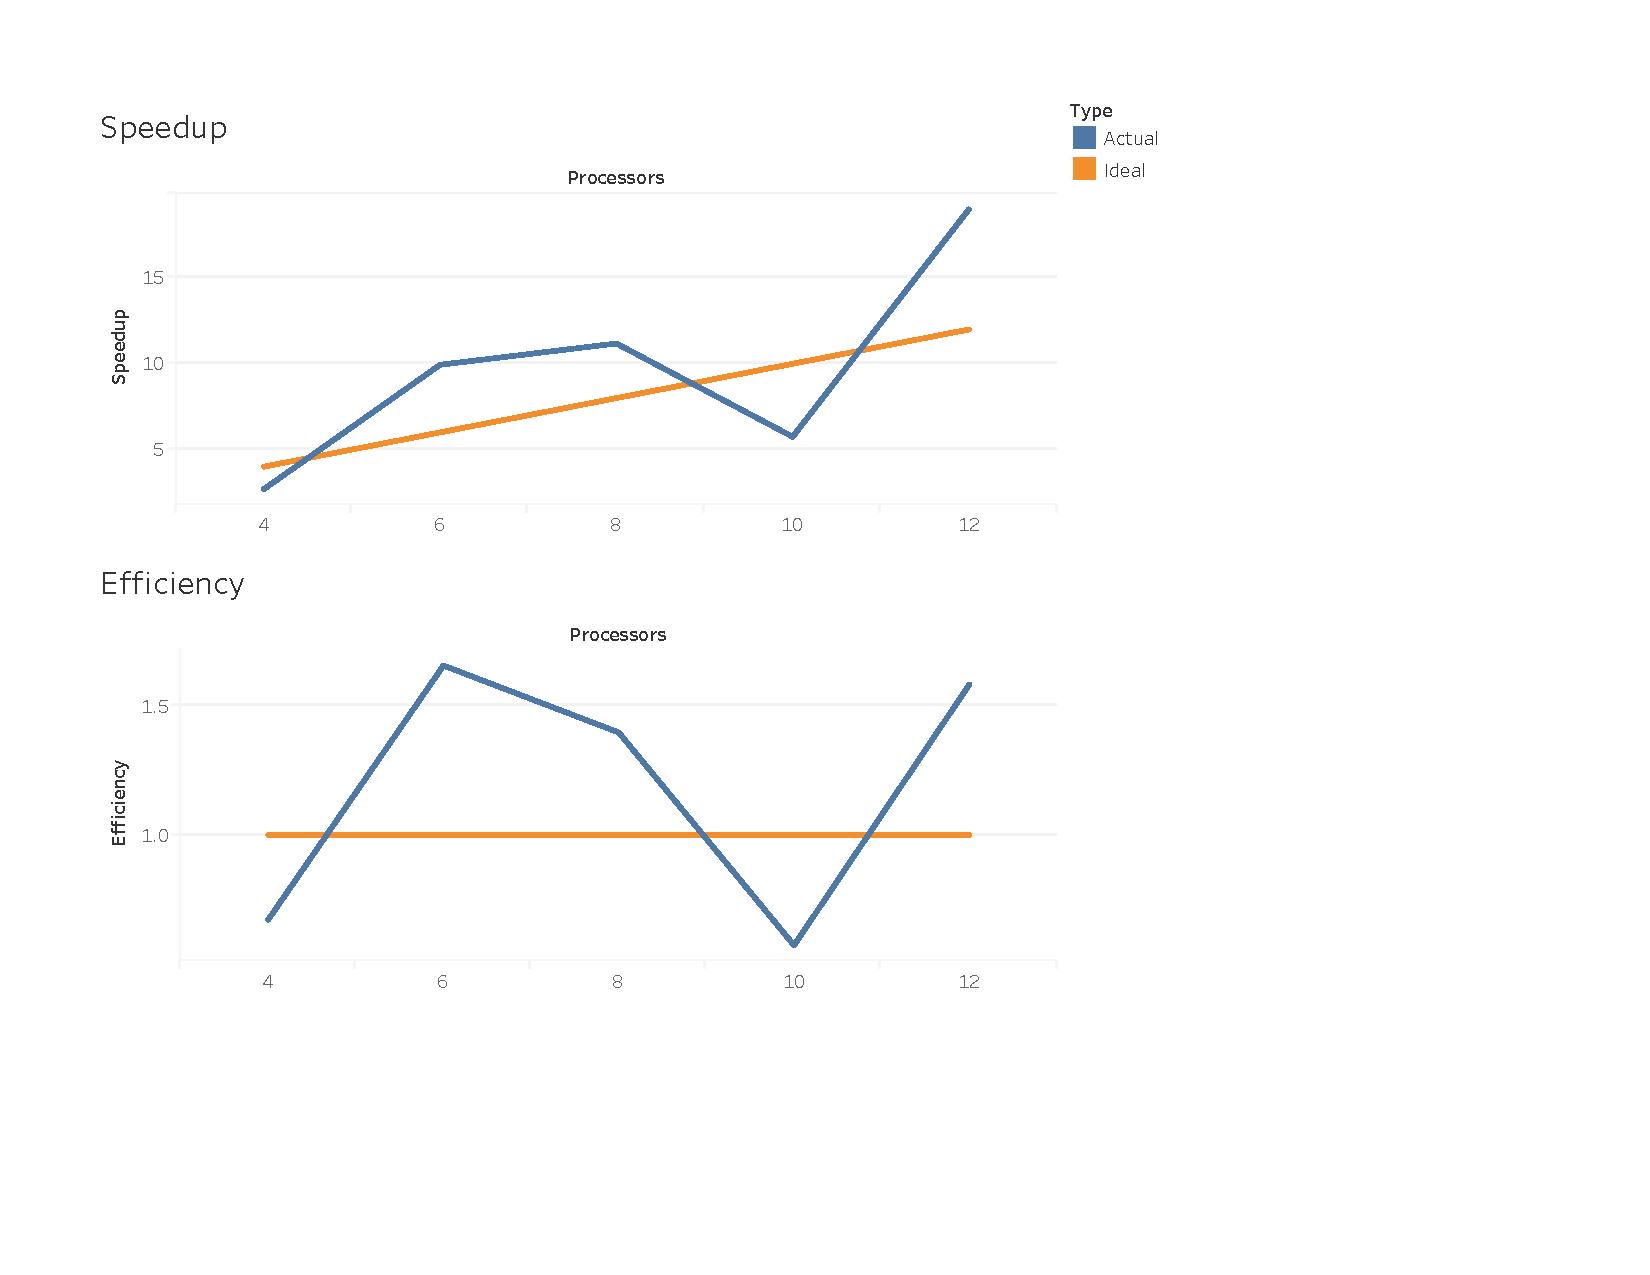
\includegraphics[height=0.8\textheight]{../../EETO/ResultAnalysis/Speedup_Efficiency.pdf}
	\caption{Speed-up and Efficiency}
\end{figure}

This graph shows the super-linearity of the parallel implementation.
So, an analysis on memory leak was done.

A sequential code with networks size 4 was run and snapshots of the objects released were captured with time difference of barely some minutes. Some object types with greater increments are shown in Figure 4.8.

Despite the fact that python comes with it's own garbage collector, this was a result of the circular reference issue, thus preventing the garbage collector from freeing the objects held in memory.The garbage collector works on the principle of reference counting algorithm.
Reference cycles can occur in container objects (lists, dictionaries, classes, tuples). The re-referencing of tuples and dictionaries of dictionaries used while saving the hyper-parameter sets were left untracked. 

\begin{figure}
	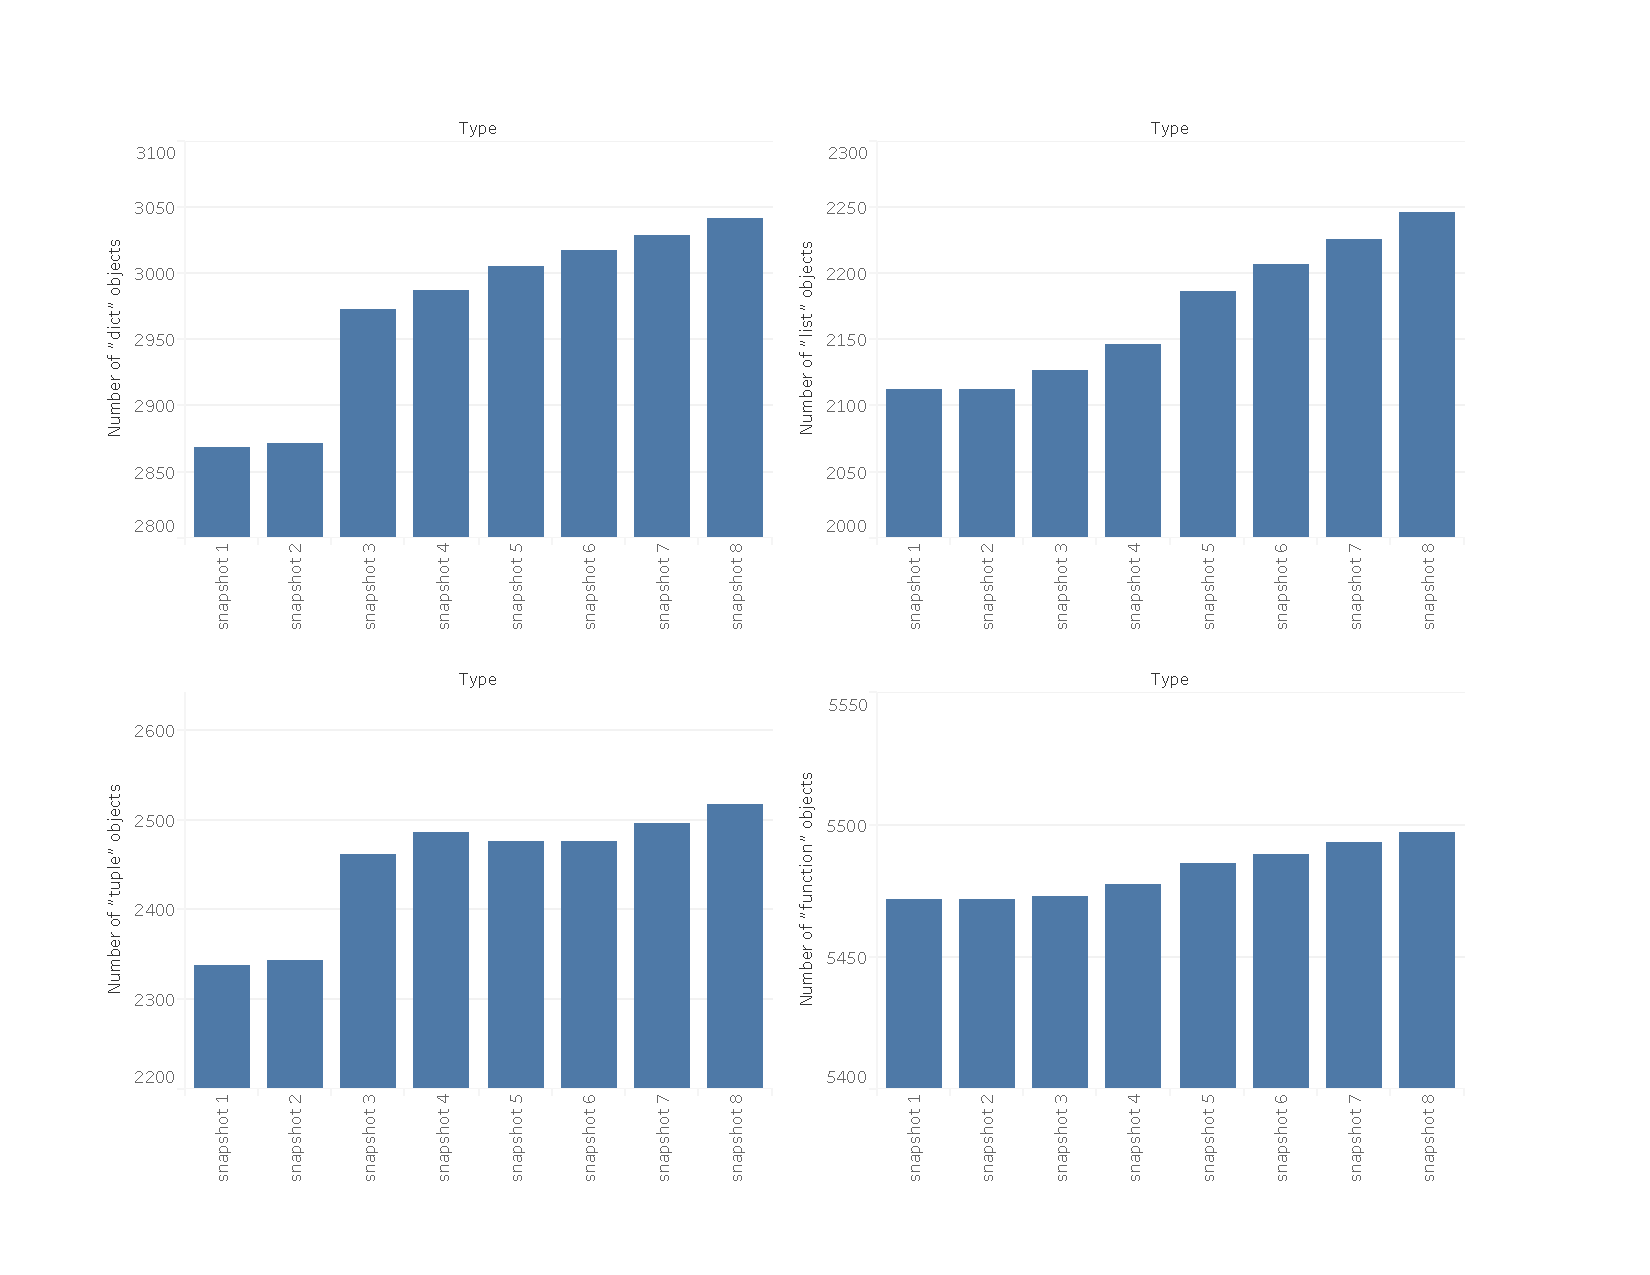
\includegraphics[width=1.25\textwidth]{../../EETO/ResultAnalysis/MemoryLeak.pdf}
	\caption{Memory leak Snapshots}
\end{figure}

From Figure 4.8, it can be easily concluded that the object type "dict", "tuple" are problematic
To further validate the same, the total number of objects and the object sizes have been looked upon as shown in Figure 4.9

\begin{figure}
	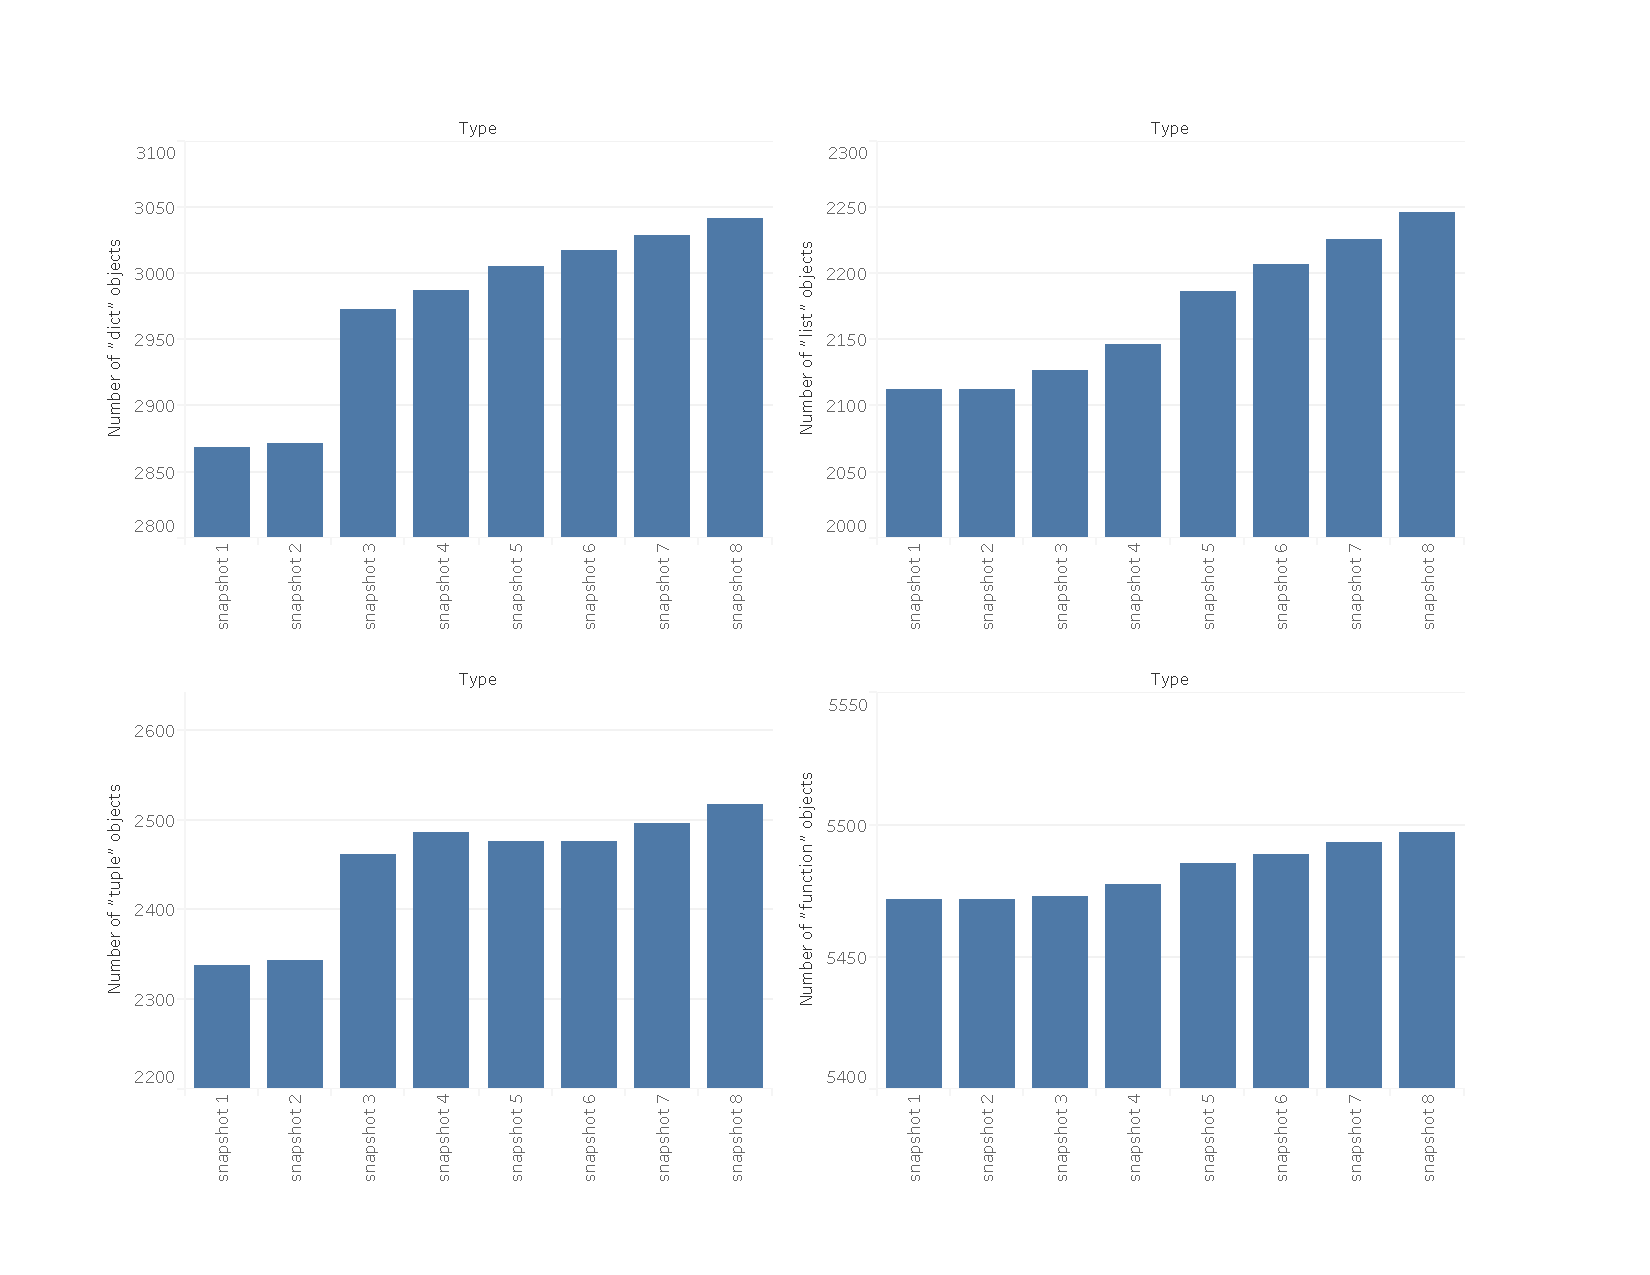
\includegraphics[width=1.1\textwidth]{../../EETO/ResultAnalysis/MemoryLeak.jpg}
	\caption{Memory leak with generations}
\end{figure}


%\clearpage

TCHPC-Boyle cluster has 32 compute nodes, providing memory/storage resources to virtual machine instances. In this thesis, most of the codes ran in boyle nodes 0-10 which have 16 cores.


\begin{tabular}{|p{3cm}||p{3cm}|p{3cm}|p{3cm}|p{3cm}| }
	\hline
	\multicolumn{5}{|c|}{Structure of Boyle cluster nodes} \\
	\hline
	\multicolumn{5}{|c|}{Memory at node and core level for each partition} \\
	\hline
	Nodes & Cores & Partition & Memory & Memory per Node\\
	\hline
	13&28&compute&128000&4571\\
	8&28&compute&256000&9143\\
	10&16&compute&64000&4000\\
	1&28&compute&128000&4571\\
	20&240&mic&7697&32\\
	1&28&long&256000&9143\\
	\hline
\end{tabular}


While creating the neural network models every generation, the keras library stores the model creation session. Because of storing all these sessions, SLURM output shows memory error. 



An analysis which was previously carried out: Parallel code using 28 cores was run on one of the 28core nodes. Memory usage of the code was more than 4.5G. Error:

\begin{verbatim}
“slurmstepd: Exceeded step memory limit at some point.”
\end{verbatim}

The solution is to clear session after usage of every model. In addition to this, although python uses automatic garbage collectors, reclaiming memory rendered useless by the code, in the code hyper-parameters are given by dictionary of a dictionary of a dictionary, which is run for all networks over number of generations, so to avoid unnecessary filled memory, the variables should be deleted or replaced with "None" value. 




\clearpage

\section{Quantum Genetics Inspired Genetics Inspired Exploration vs Exploitation based Optimization for Neural Network Tuning}



A comparison of fitness with evolving generations can be seen in Figure 4.10. 
The highest fitness achieved is 39.18\% (~10\% lesser than what was achieved without Quantum Inspired Algorithm). Thus proving that initializing the networks with more randomized values did not turn out fruitful. 


The graph shows the best fitness achieved for different network types at generation level. With 4 networks, the best fitness is not achieved even after 25 generations, but is continuously improving, thereby demanding more generations to be run. The graph proves that with increment in number of networks the the chances of getting better fitness in initial generations increases.


\begin{figure}
	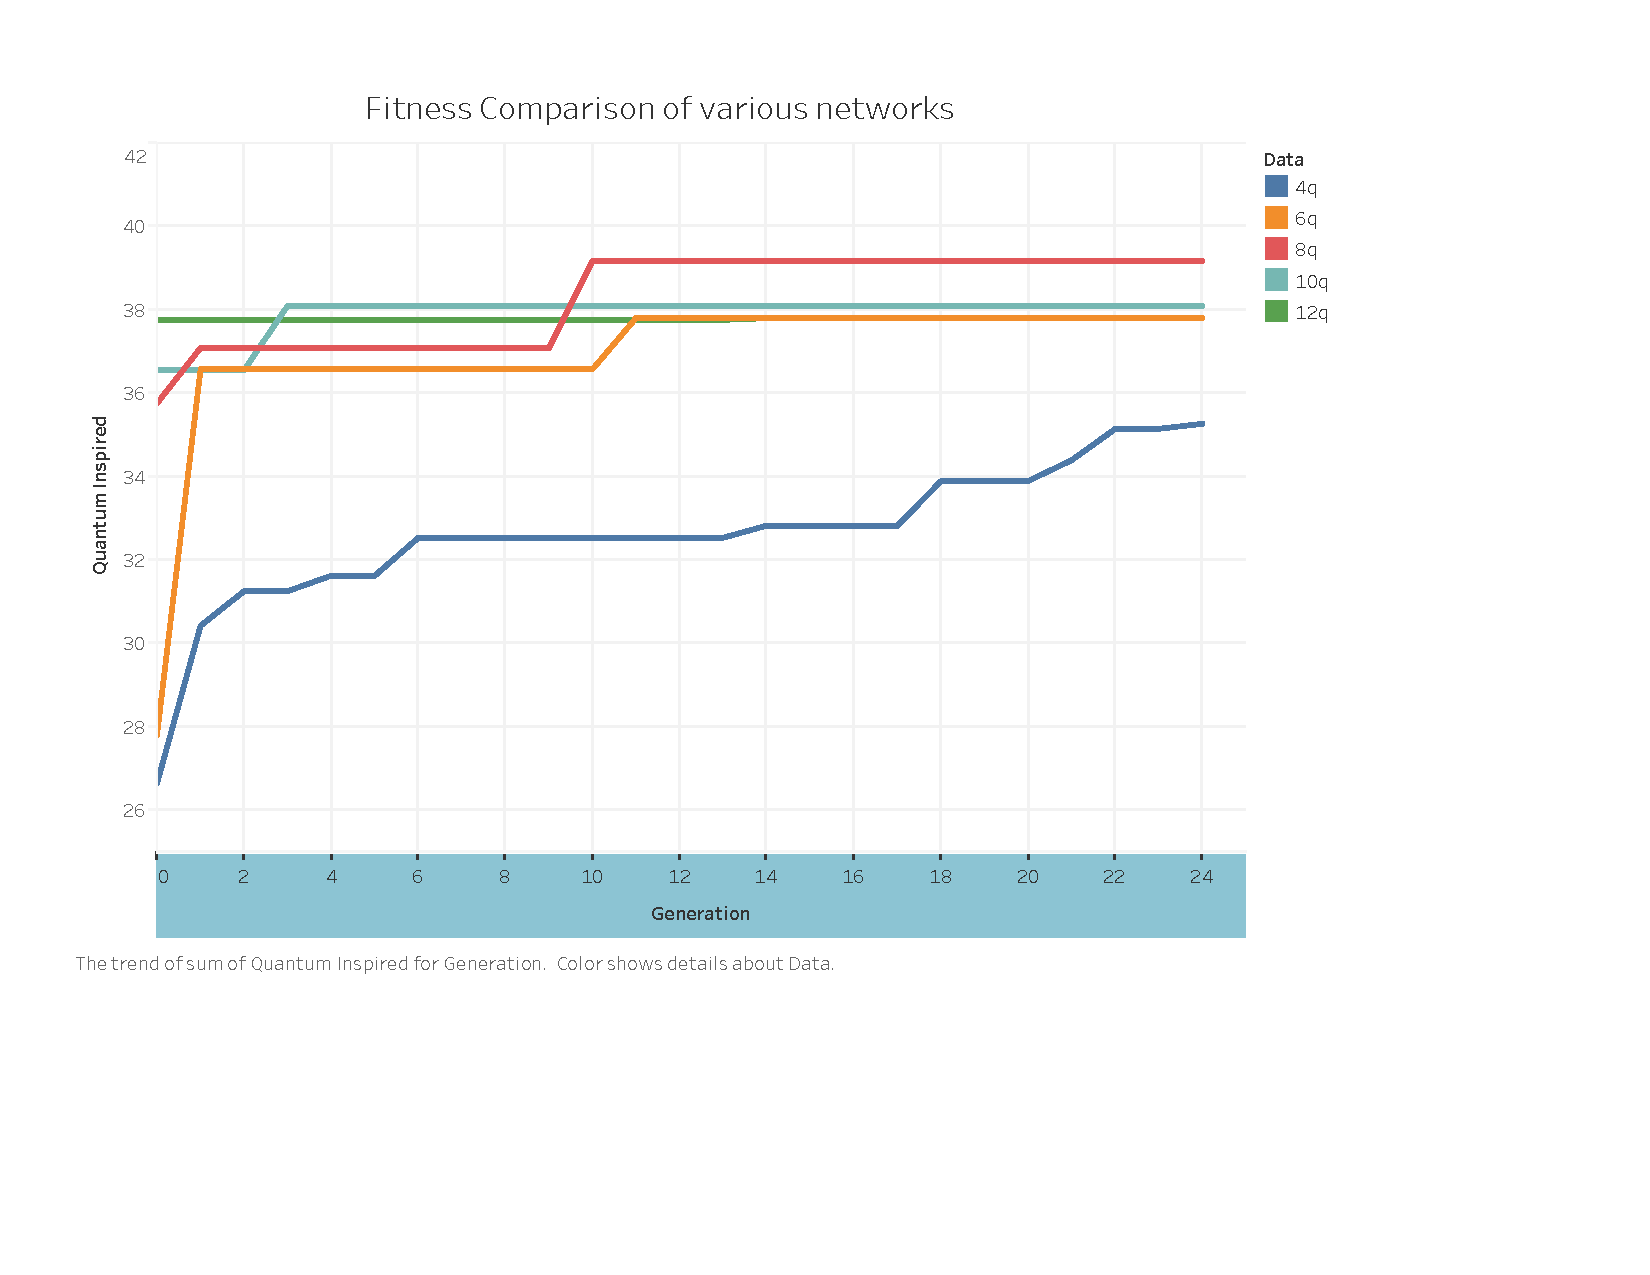
\includegraphics[width=1.4\textwidth]{../../EETO/ResultAnalysis/QEETO/Fitness.pdf}
	\caption{Best fitness achieved - for every generation for various network sizes; \newline Legend Decode: \newline 4q -> 4 Networks Quantum Inspired Algorithm Data; \newline 6q -> 6 Networks Quantum Inspired Algorithm Data;\newline 8q -> 8 Networks Quantum Inspired Algorithm Data; \newline 10q -> 10 Networks Quantum Inspired Algorithm Data; \newline 12q -> 12 Networks Quantum Inspired Algorithm Data; }
\end{figure}


A quick comparison has been done taking 4 networks for the parallel implementation done in previous section vs the implementation done using Quantum Inspired Algorithm for time taken as well as the fitness evolution as shown in Figure 4.11

\begin{figure}
	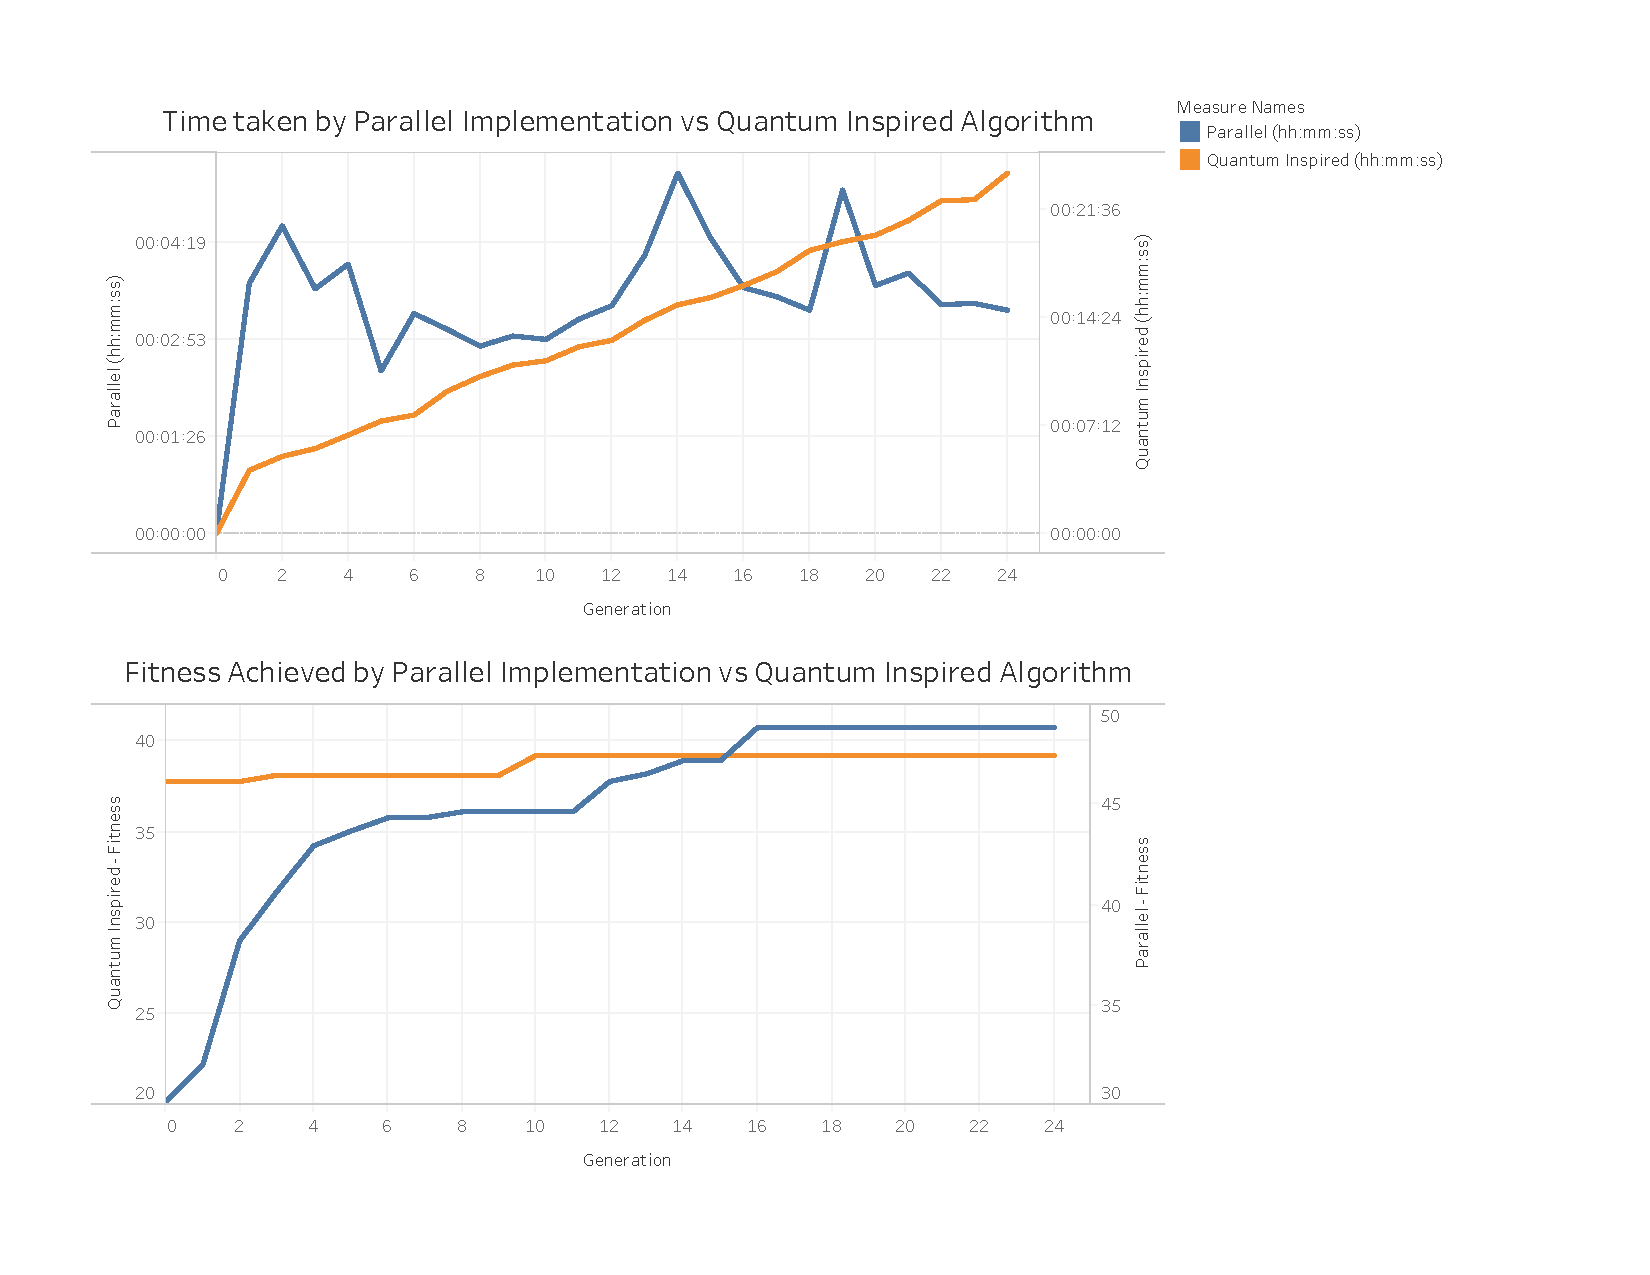
\includegraphics[height=0.7\textheight]{../../EETO/ResultAnalysis/QEETO/OverallComparison.pdf}
	\caption{The graph shows time taken and fitness comparison taking 4 networks \newline a. the time taken in both Parallel vs Quantum Inspired Algorithm implementations \newline b. best fitness for every generation in both Parallel vs Quantum Inspired Algorithm implementations }
\end{figure}


It can be easily inferred that time taken in Quantum Inspired Algorithm increases with generation as a result of memory leak. In case of parallel code, the time taken increases and reduces thereby contributing to more number of cores being used and increment in time is a result of heavier network (network demanding more computation because of hyper-paramenter selection) being trained.




\chapter{Summary}


In this thesis, Cifar10 image classification dataset is used. Four optimization methods have been implemented to get the best set of hyper-parameters, which are:
\begin{enumerate}
	\item Sequential Genetic Inspired Algorithm
	\item Single Population Fine Grained Algorithms
	\item Multiple-population Coarse Grained Algorithms (Island Model)
	\item Quantum Inspired Algorithm
\end{enumerate}


These methods have been run and tested on various network sizes (4, 6, 8, 10 and 12). 

Overall, highest efficiency fetched is 51.14\% from parallel code giving best set of hyper-parameters as follows: \newline \newline \textbf{adamax (Optimizer) - elu (Activation function) - 128 nodes - 3 layers - 0.1 dropout} \newline \newline 
This accuracy is a result of parent fitness. Also, there is a minute difference between the efficiencies of parallel and serial methods with best efficiency achieved from running serial code to be 49.05 using hyper-parameter which similar to the overall best hyper-parameter set as: \newline \newline \textbf{adamax (Optimizer) - elu (Activation function) - 128 nodes - 9 layers - 0.1 dropout}. 

The difference is in the number of layers, which is another interesting result: the decrease in layers and the increase in neurons in hidden layers are two major factors resulting in higher frequencies.


There have been cases where child fitness is higher than it's parent's thereby confirming the chances of better exploration and getting out of the local maxima. However, the best efficiencies from all the methodologies sequential (49.05\%), parallel (51.14\%) and quantum inspired (39.18\%) code have been achieved as a result of parent fitness.


Also, networks despite same hyper-parameter configurations take different time in training resulting in different accuracy/efficiency. However, the difference in time and accuracy is not high and can be ignored (time difference ~ 4-5 minutes in serial code, accuracy difference ~ 1-2\%)


Different sets of hyper-parameters took different time e.g. hyper-parameter set with larger number of nodes (say 128) resulted in increased time taken to train the network as compared to the set with smaller number of nodes(say 4).


Although, python supports garbage collection, the parallel code has shown super-linear speed-up. This is because of huge memory leak: ~50MB in 5 generations. The same if computed for hundreds of generations will fail.



In all the algorithms, it was seen that crossover and mutation steps took seconds to complete, on the contrary, fitness evaluation using keras took several minutes to complete. 


 
Furthermore, out of all the implementations parallel code is time and resource efficient (island model being better of the two parallel implementations). The Parallel Algorithms have resulted in decreased time taken for the computationally expensive neural network tuning.


%\input{background/background.tex}
%\input{project/project.tex}
%\input{evaluation/evaluation.tex}
%\input{conclusion/conclusion.tex}
\bibliographystyle{unsrtnat}
\bibliography{bibs/sample}
%\appendix
%\renewcommand{\thechapter}{A\arabic{chapter}}
%\input{appendix/appendix.tex}


\end{document}